% This is a LaTeX thesis template for Monash University.
% to be used with Rmarkdown
% This template was produced by Rob Hyndman
% Version: 6 September 2016

\documentclass{monashthesis}

%%%%%%%%%%%%%%%%%%%%%%%%%%%%%%%%%%%%%%%%%%%%%%%%%%%%%%%%%%%%%%%
% Add any LaTeX packages and other preamble here if required
\usepackage{subcaption}
\usepackage{lscape}
%%%%%%%%%%%%%%%%%%%%%%%%%%%%%%%%%%%%%%%%%%%%%%%%%%%%%%%%%%%%%%%

\author{Dewi Lestari Amaliah}
\title{Visualising Multilevel Regression and Poststratification: Alternatives to the Current Practice}
\studentid{31251587}
\def\degreetitle{Master of Business Analytics}
% Add subject and keywords below
\hypersetup{
     %pdfsubject={The Subject},
     %pdfkeywords={Some Keywords},
     pdfauthor={Dewi Lestari Amaliah},
     pdftitle={Visualising Multilevel Regression and Poststratification: Alternatives to the Current Practice},
     pdfproducer={Bookdown with LaTeX}
}


\bibliography{thesisrefs}

\begin{document}

\pagenumbering{roman}

\titlepage

{\setstretch{1.2}\sf\tighttoc\doublespacing}

\clearpage\pagenumbering{arabic}\setcounter{page}{0}

\hypertarget{abstract}{%
\chapter*{Abstract}\label{abstract}}
\addcontentsline{toc}{chapter}{Abstract}

Conducting a large survey to provide statistics to subpopulation levels is expensive, time-consuming, and often comes with unrepresentative samples. Multilevel Regression and Poststratification (MRP) has been a promising method to provide reliable estimates for subpopulations. To current, graphical display is widely used to communicate and diagnose MRP estimates. However, there have been few studies on how visualisation should be performed in this field. Accordingly, this study tries to fill this gap by examining the current practice of MRP visualisation using a systematic literature review. This study also applies MRP to estimate the Trump vote share in the U.S. 2016 presidential election using the Cooperative Congressional Election Study (CCES) to demonstrate the implication of the current visualisation practice and explore alternatives for its improvement. The main finding of this study is that uncertainty is not widely displayed in the current practice. The choropleth map is the most frequently used to display MRP estimates even though it only shows point estimates and could hinder the information from areas with a small polygon. Uncertainty is also not much displayed for model diagnostic in the current practice. Using various graphical representations, this study shows that visualisation with uncertainty can illustrate the effect of different model specifications on the estimation result. In addition, this study also proposes an alternative graph to also take the bias-variance trade-off into account in evaluating MRP performance.

\newpage

\hypertarget{acknowledgements}{%
\chapter*{Acknowledgements}\label{acknowledgements}}
\addcontentsline{toc}{chapter}{Acknowledgements}

I would like to express my deepest gratitude to my supervisors, Lauren Kennedy and Shiro Kuriwaki. They have given me so much time, knowledge, wisdom, and patience since I started until I finished this thesis. Their continuous feedback, guidance, encouragement, and advice were like a light in the dark, especially when this thesis became increasingly challenging to complete.

I would like to extend my gratitude to Dan Simpson, the chief examiner of Master of Business Analytics and Creative Activity, for all the guidance in completing this unit.

Last but not least, I would like to thank Australia Awards Scholarship for giving me the scholarship to study at the Monash University. Without it, studying in Australia would only remain as one of my childhood dreams.

\hypertarget{r-packages}{%
\section*{R packages}\label{r-packages}}
\addcontentsline{toc}{section}{R packages}

Several R \autocite{R} packages are utilized to produce this thesis: mrpkit \autocite{mrpkit}; ccesMRPprep \autocite{ccesmrpprep}; brms \autocite{brms}; survey \autocite{survey}; tidyverse \autocite{tidyverse}; forcats \autocite{forcats}; Metrics \autocite{Metrics}; data.table \autocite{datatable}; kableExtra \autocite{kable}; janitor \autocite{janitor}; scales \autocite{scales}; ggplot2 \autocite{ggplot2}; patchwork \autocite{pw}; flipPlots \autocite{flipflops}; igraph \autocite{igraph}; urbnmapr \autocite{urban}; ggstance \autocite{stance}; ggpmisc \autocite{ggpmisc}; wacolors \autocite{wacolors}; rmarkdown \autocite{rmd}; knitr \autocite{knitr}; MonashEBSTemplates \autocite{monashtemp}.

\hypertarget{ch:intro}{%
\chapter{Introduction}\label{ch:intro}}

An accurate estimate of subpopulations is essential to draw insight from the data, especially when policy or decision is made in small area levels. However, conducting a large survey to provide statistics of subpopulations is expensive, time-consuming, and sometimes comes with unrepresentative samples. Multilevel regression and poststratification, henceforth referred to as MRP, is a model-based approach deemed to estimate subpopulation reliably. In short, MRP incorporates a multilevel regression technique to predict the outcome of interest using survey data. This prediction is then poststratified using the population size from a larger survey or census to get the population estimates.

MRP is widely applied to do small area estimation in the absence of a subnational survey \autocite{hanretty}. In this case, MRP is able to estimates small geographic areas, such as state or county estimates. MRP also allows the demographic-wise estimation, such as estimation by gender, age group, and education. Additionally, MRP is also often applied to adjust the estimation from the non-representative survey as a result of the difficulties in recruiting representative survey respondents \autocite{mrp-book}.

The standard method to communicate and validate the MRP estimates, such as their accuracy, is by using graphics. Indeed, statistical graphics are regarded a powerful tool to communicate quantitative information and analyse data \autocite{ClevelandWilliamS,1983Gmfd}. \textcite{WickhamHadley2015VsmR} state that statistical visualisation, particularly model visualisation, is imperative as it helps us to understand the model better, for example, how the model changes as its parameters change or how the parameters change as the data change. They also mention that model visualisation is important to show the model's goodness of fit and whether it is good for some regions only and worse in other regions, or it is uniformly good.

While visualisation is common to communicate and diagnose MRP models, only a few discussions and studies on how should be it performed. Two of the studies that nearly intersect with this topic were conducted by \textcite{mekelagelman} and \textcite{saundra}. However, \textcite{mekelagelman} only focus on a graphical method for discovery and communication purposes of polling results. Besides, the MRP visualisations that they display as examples are isolated on Gelman's previous papers only. Meanwhile, the latter study by \textcite{saundra} only focuses on how the graphics in public opinion research should be displayed. Therefore, this study tries to fill the gap by discussing the current practices of MRP visualisations generally, not only in public opinion and polling estimates scopes. It also aims to explore the possible alternative improvements to those current practice.

Explicitly, the objectives of this study are:

\begin{enumerate}
\def\labelenumi{\arabic{enumi}.}
\tightlist
\item
  Discuss the current practice of visualisation of MRP models.
\item
  Understand the implication of existing visualisation choices with real-world data.
\item
  Explore possible improvements of the current practice of MRP visualisation.
\end{enumerate}

The first objectives will be reached by doing a systematic literature review, while the second and the third goals will be demonstrated through a case study.

\hypertarget{overview}{%
\section{MRP Overview}\label{overview}}

MRP is essentially conducted with two stages, i.e., multilevel/hierarchical regression modeling and poststratification. The idea is to combine model-based estimation commonly used in small area estimation with poststratification, which is considered the general framework as a weighting scheme in survey analysis \autocite{Gelman97poststratificationinto}. They further argue that using multilevel regression estimates for poststratification allows the estimation for many more categories to gain more detailed population information.

Formally, let \(K\) be the number of categorical variables in the population and the \(k_{th}\) has \(J_k\) categories/levels, the population can be then expressed as \(J = \prod_{k=1}^K J_k\) cells. For every cell, there is a known population size \(N_j\). If the variable in the population is not in categorical form, then it should be categorised first. Next, suppose that the outcome of interest is a binary variable. MRP procedure is summarised in two stages as follows \autocite{GaoYuxiang2021IMRa}:

\begin{enumerate}
\def\labelenumi{\arabic{enumi}.}
\tightlist
\item
  \textbf{Multilevel regression stage}. Multilevel regression is fitted to get estimated population averages \(\theta_j\) for every cell \(j \in \{1, ...., J\}\). The multilevel logistic regression has a set of random effects \(\alpha^k_{m[j]}\) for each categorical covariate \(k\). These random effects have the effect of pooling each \(\theta_j\) partially towards \(X_j\beta\), the \(j_{th}\) is the row of \(\textbf{X}\), the design matrix corresponding to \(\theta_j\), while \(\beta\) is the fixed effect of the model. Suppose that \(n\) is the number of individual observations in the survey data, the form of multilevel regression could be written as follows:
\end{enumerate}

\begin{equation} 
\begin{split}
& Pr(y_i = 1) = logit^{-1}\left(X_i\beta + \sum^K_{k=1}\alpha^k_m[i]\right), for\ i=1, ..., n,\\
& \alpha^k_m \sim N(0, \sigma^2_k), for\ m = 1, ..., M_k
\end{split}
\label{eq:mrp-stage1}
\end{equation}

\begin{enumerate}
\def\labelenumi{\arabic{enumi}.}
\setcounter{enumi}{1}
\tightlist
\item
  \textbf{Poststratification stage}. The probabilities of the outcome from the previous stage, \(\theta_j\), is then poststratified using the known population size \(N_j\) of each cell \(j\) to get the estimates at the subpopulation level. This stage corrects the nonresponse in the population by utilizing the known size of every cell \(j\) relative to the total population size \(N = \sum_{j=1}^J N_j\). In other words, the estimates is a weighted average of \(\theta_j\) with \(N_j\) as the weight. Suppose that \(S\) is the subpopulation which is the combination of categories in the poststratification matrix, the MRP estimates could be expressed as:
\end{enumerate}

\begin{equation} 
\begin{split}
\theta_S = \frac{\sum_{j \in S}N_j\theta_j}{\sum_{j\in S}N_j}
\end{split}
\label{eq:mrp-stage2}
\end{equation}

\hypertarget{thesis-structure}{%
\section{Thesis Structure}\label{thesis-structure}}

This thesis is structured as follows:

\begin{itemize}
\item
  Chapter \ref{ch:syslitrev} is a systematic literature review. This chapter discuss the review of current practice in MRP visualisations in various studies.
\item
  Chapter \ref{ch:case-stud} is a case study of MRP visualisations. This chapter aims to demonstrate the MRP application in the case of U.S. presidential voting result estimation. This chapter also demonstrates how the current practice of MRP visualisation could be improved.
\item
  The final chapter, Chapter \ref{ch:conclusion}, summarises the findings and concludes the contribution of this study and possible future works.
\end{itemize}

\hypertarget{ch:syslitrev}{%
\chapter{Systematic Literature Review}\label{ch:syslitrev}}

This study is performed using a systematic review method. This method collects empirical evidence explicitly and systematically using pre-specified eligibility criteria to answer a specific research question \autocite{cochrane}. Systematic literature reviews also enable the process of finding the gap in a field of science, such as understanding what has been done and what needs to be done \autocite{LinnenlueckeMartinaK2020Cslr}. Hence, in this case, systematic literature review could assist us to understand the common practice in MRP visualisations so that we can explore how to improve.

According to \textcite{brown_uni}, the key criteria of the systematic literature review are: \emph{``a clearly defined question with inclusion \& exclusion criteria; rigorous \& systematic search of the literature; critical appraisal of included studies; data extraction and management; analysis \& interpretation of results; and report for publication.''} Hence, to conform with these criteria, this study incorporates the Preferred Reporting Items for Systematic Reviews and Meta-Analysis (PRISMA)'s checklist and flow diagram. The following subsections discuss the steps conducted following these criteria.

\hypertarget{literature-identification}{%
\section{Literature Identification}\label{literature-identification}}

MRP is applied in various scientific fields, ranging from social and political science to public health. Therefore, to identify relevant literature, this study refers to research databases instead of field-specific journals. Those databases are JSTOR, EBSCO, and PubMed. The first two databases are chosen due to their broad range of field coverage, while the latter is chosen since MRP is sometimes also applied in the health and medical fields. These databases were also chosen to represent the heterogeneity of the field, which is one of the important factors in a systematic literature review \autocite{SchweizerMarinL2017Apgt}.

From these databases we identify relevant articles using the combination of several search terms. Generally the search terms include the term ``multilevel regression'', ``post-stratification'', ``poststratification'', and ``multilevel model''. Our target literature is articles that are written in English. We exclude all of the publications before 1997 since this was the first proposal date for MRP. Initially we included only the title/abstract when searching these databases. However, using this method limits the set of potential articles to only include those with the search term in the abstract/title. To rectify this, we also include a search with ``all field'' in the search criteria. Note that for EBSCO, we directly apply the search for all fields. The detailed literature identification is shown in Table \ref{tab:search-term}.

The total number of articles from this search criteria are 327. Next, we utilize the literature manager, EndNote X9, to manage these articles and to find duplicate articles. After removing those duplicate articles, we have 212 articles to be screened in the next stage.

\begin{landscape}\begin{table}

\caption{\label{tab:search-term}Detail of literature identification}
\centering
\resizebox{\linewidth}{!}{
\begin{tabular}[t]{l>{\raggedright\arraybackslash}p{15em}lllr}
\toprule
Database & Search Terms & Search Field & Inclusion & Exclusion & Number Returned\\
\midrule
JSTOR & (multilevel regression and poststratification) OR (“post-stratification”) & Abstract & Article, content I can access, English & anything before 1997 & 44\\
JSTOR & (("multilevel regression" AND ("post-stratification" OR Poststratification)) OR ("multilevel model" AND ("post-stratification" OR Poststratification))) & All field & Article, English & anything before 1997 & 142\\
EBSCO & "multilevel regression with post-stratification" OR "multilevel regression with poststratification" OR "multilevel regression and Poststratification" OR "multilevel regression and Post-stratification" & All field & Academic (Peer-Reviewed) Journals, English & anything before 1997 & 42\\
EBSCO & (multilevel regression AND post-stratification) OR (multilevel model AND post-stratification) OR (multilevel regression AND poststratification ) OR (multilevel model AND poststratification) & All field & Academic (Peer-Reviewed) Journals, English & anything before 1997 & 45\\
PubMed & "multilevel regression with post-stratification" OR "multilevel regression with poststratification" OR "multilevel regression and Poststratification" OR "multilevel regression and Post-stratification" & Title/Abstract & Article, English & anything before 1997 & 26\\
\addlinespace
PubMed & (multilevel regression AND post-stratification) OR (multilevel model AND post-stratification) OR (multilevel regression AND poststratification) OR (multilevel model AND poststratification) & All field & Article, English & anything before 1997 & 28\\
\bottomrule
\end{tabular}}
\end{table}
\end{landscape}

\hypertarget{screening-and-eligibility-criteria}{%
\section{Screening and Eligibility Criteria}\label{screening-and-eligibility-criteria}}

We screen all of the articles based on predetermined criteria. We find that 3 articles are apparently not research papers. This results in 209 abstracts to be screened. To screen efficiently, we use two stages. The first stage is a review of abstracts, the second a full manuscript review.

\hypertarget{stage-1-review-of-abstracts}{%
\subsection{Stage 1: Review of abstracts}\label{stage-1-review-of-abstracts}}

In the first stage DA and LK independently review all article abstracts with the following eligibility criteria:

\begin{enumerate}
\def\labelenumi{\arabic{enumi}.}
\tightlist
\item
  The abstract should mention analysis of data or creation of simulation data.
\item
  The abstract should mention the use of MRP or multilevel models to make population estimates or the use of other regression models (BART, spatial, stacking, trees) to make population estimates.
\end{enumerate}

During the screening, DA and LK agreed that 61 articles meet the eligibility criteria listed above, while 104 articles do not meet the criteria. The two reviewers disagreed on 44 articles. Accordingly, DA and LK skim the full manuscript to decide whether the paper could be included in the next stage or not. As the result, an additional 22 more articles are moved to stage 2, making a total of 83.

\hypertarget{stage-2-full-manuscript-review}{%
\subsection{Stage 2: Full manuscript review}\label{stage-2-full-manuscript-review}}

DA reviews the full manuscript on 83 articles based on a second set of criteria. The aim of this stage is to get the list of the final articles that would be included in the study. We set the criteria of inclusion as follow:

\begin{enumerate}
\def\labelenumi{\arabic{enumi}.}
\tightlist
\item
  It should apply MRP as its method.
\item
  It should contain at least one plot relate to MRP findings.
\end{enumerate}

During this stage, we exclude 4 articles as they do not meet the first criteria. Further, 7 articles are excluded as they do not meet the second criteria. Also, an article is not included because it is a duplicate that was not detected automatically by Endnote X9. Finally, we have 71 articles to be reviewed in the next stage. Figure \ref{fig:prisma-flowchart} displays the PRISMA flow chart of this study. This figure is generated using \texttt{PRISMA2020} \autocite{prisma2020}.

\begin{figure}
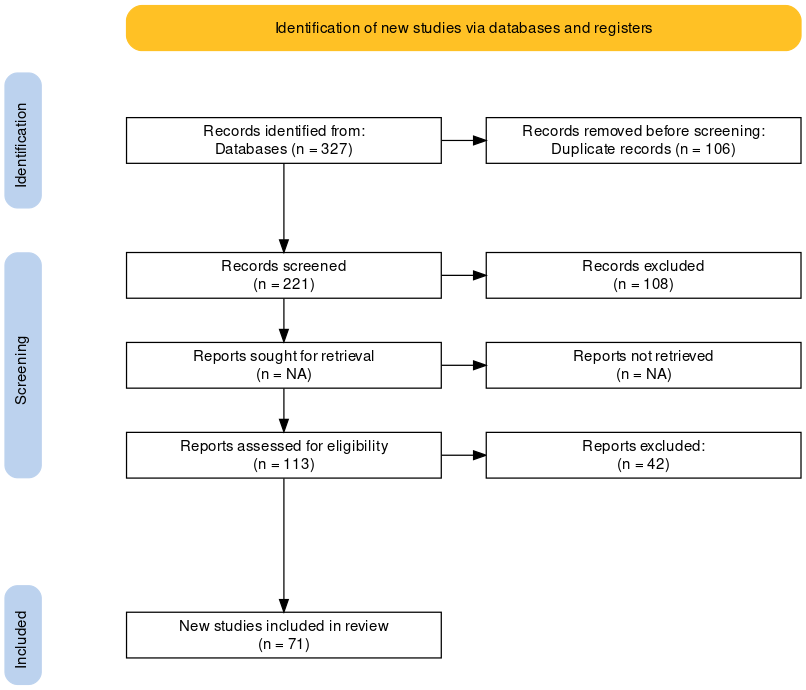
\includegraphics[width=0.9\linewidth]{figures/prisma_fc} \caption{PRISMA flow chart of this systematic literature review.}\label{fig:prisma-flowchart}
\end{figure}

\hypertarget{data-extraction-and-analysis}{%
\section{Data Extraction and Analysis}\label{data-extraction-and-analysis}}

We focus the data extraction on the MRP-related plot. We manually create a metadata for each plot (included in the supplementary material). We will use this metadata to analyse the current reporting practices with MRP. This metadata will also ensure the reproducibility of the analysis and to maintain the transparency of the systematic literature review process.

We code the plots according to their type, i.e., communication (coded to 0) and diagnostic plot (coded to 1). For diagnostic plots, we examine whether the plots compare MRP with other estimates, which are:

\begin{enumerate}
\def\labelenumi{\arabic{enumi}.}
\tightlist
\item
  Raw (direct estimates or direct disaggregation);
\item
  Ground truth;
\item
  Weighted estimates;
\item
  Estimates from other MRP models, for example, a paper build several MRP models from various simulation scenarios or using different covariates;
\item
  Estimates from another study/survey;
\item
  Estimates from another method, for example comparing MRP with Bayesian Additive Tress with Post-Stratification(BARP).
\end{enumerate}

Plots that show a comparison of MRP with the above list would be coded to 1, otherwise coded to 0.
Diagnostic plots also categorised based on how they compare the performance of MRP. The five observed criteria are:

\begin{enumerate}
\def\labelenumi{\arabic{enumi}.}
\tightlist
\item
  Bias;
\item
  Mean Absolute Error (MAE);
\item
  Mean Square Error (MSE)/ Relative Mean Square Error (RMSE);
\item
  Standard Error (SE);
\item
  Correlation.
\end{enumerate}

Each plot is assessed based on the use of the performance metric. For each metric is scored based on whether it is used (coded 1) or not (coded 0).

We also review other features of the plot using the grammar in \texttt{ggplot2} \autocite{ggplot2} as a framework. The common grammar used in practice allows us to understand to what extend MRP models are effectively visualised. It is worth noting that there is no specific convention or well-documented recommendation on how data should be visualised as building a graph more often involves choice or preference \autocite{MIDWAY2020100141}. For example, there is no specific convention on which variable should be put on the x and y-axis in a scatter plot, even though it has been common knowledge to put the response variable on the y-axis and the explanatory variable on the x-axis. Hence, grammar assists us in evaluating well-formed graphics \autocite{layered-grammar}. In addition, \textcite{vanderplas} mention that classifying and comparing graphs according to their grammar is more robust and more elegant.

Accordingly, we examine the facet, geom, axis, color, and shape. For reproducibility, the metadata also contains the article's author/s, publication year, title, and corresponding figure number as it appeared in the article. After the extraction, we analyze the data using graphical visualization with \texttt{ggplot2} \autocite{ggplot2}. The result will be discussed in the following subsection.

\hypertarget{com-prac}{%
\section{Common practices in MRP visualisations}\label{com-prac}}

In this study, graphics are classified into two types, i.e., communication and diagnostic plots. A plot is classified as a communication plot if the plot's goal is solely to convey the MRP result. A diagnostic plot is used to understand the MRP estimate, and typically displays the MRP estimation by showing the performance metrics or compares it with other estimation methods. From 71 articles, we extract the data of 243 plots. 47.33 \% of these plots are diagnostics plots, while the remaining are communication plots.

\hypertarget{performance-metrics-used-in-mrp}{%
\subsection{Performance metrics used in MRP}\label{performance-metrics-used-in-mrp}}

According to \textcite{BotchkarevAlexei2019ANTD}, performance metrics is \emph{``a logical and mathematical construct designed to measure how close are the actual results from what has been expected or predicted''} RMSE and MAE are among the most common methods used in many studies \autocite{BotchkarevAlexei2019ANTD}. However, \textcite{WillmottCJ2005Aotm} states that RMSE should not be reported in any studies since it could be multi-interpreted because it does not describe average error alone and MAE is more appropriate metric. This argument is denied by \textcite{ChaiT2014Rmse} who argue that RMSE is not ambiguous and better than MAE if the distribution of model's error is normal. Accordingly, there is no single metric that fits all methods \autocite{ChaiT2014Rmse}.

\begin{figure}
\centering
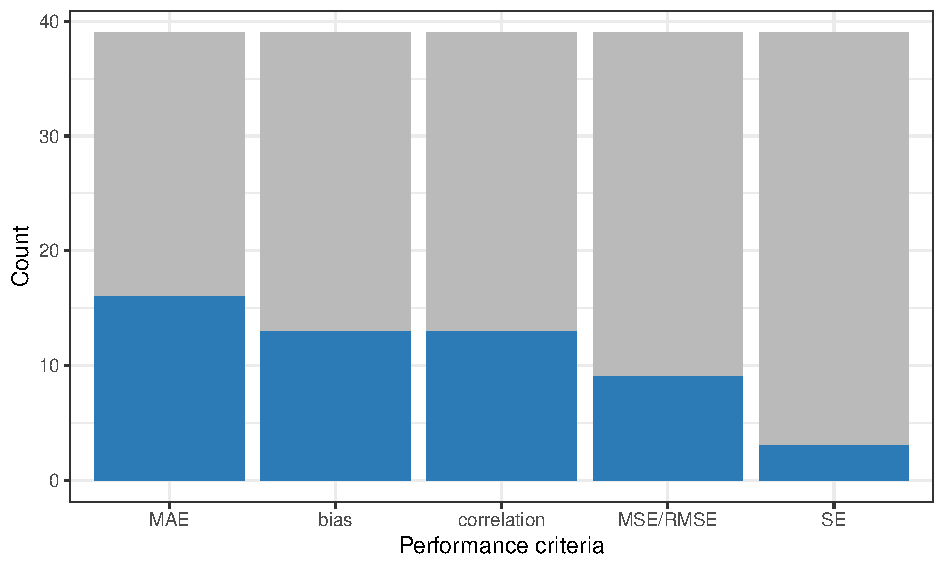
\includegraphics{thesis_files/figure-latex/perform-plot-1.pdf}
\caption{\label{fig:perform-plot}We observed five performance metrics used: Mean Absolute Error (MAE), bias, correlation, Mean Square Error/Root Mean Square Error (MSE/RMSE), and Standard Error (SE). The blue shade represents the number of articles that show performace metrics in plot, while the grey shade represents the number of articles that show performance of MRP but did not use the corresponding metrics.}
\end{figure}

In this study, we find that there are 39 plots out of 115 diagnostic plots (about 34\%) that display performance measures. As seen in Figure \ref{fig:perform-plot}, we find that MAE is the most widely used performance metric in MRP visualisations. Bias, which is interpreted similarly to MAE, is also widely used. Meanwhile, the squared error measures, which are MSE/RMSE and standard error, are only used in a few plots. It is interesting that correlation, which is not a common metric for performance, is more widely used than square error metrics.

Most of these metrics only refer to point estimates, i.e., the distance between the predicted value and the actual values. Also, these metrics mainly measure bias. However, MRP is a model in which bias-variance is applied. Therefore, other measures are also needed that reflect the degree of uncertainty and variations in the predicted value. Measures such as length of confidence or credibility interval can be used, in which the narrower the value, the more precise the estimates.

\hypertarget{common-comparisions-with-mrp}{%
\subsection{Common comparisions with MRP}\label{common-comparisions-with-mrp}}

The goal of MRP is to make a population estimate. The method aims to adjust an unrepresentative survey to obtain accurate population and sub-population estimates. Where possible MRP is usually compared with a true value. This is generally only possible in political science applications where an election provides this true estimate. To understand how MRP improves estimates from an unrepresentative survey when compared with no adjustment, MRP estimates are usually compared with direct estimates (raw). Similarly, to understand the improvement of estimates when compared with more traditional methods, MRP is often compared with weighted estimates.

\begin{figure}
\centering
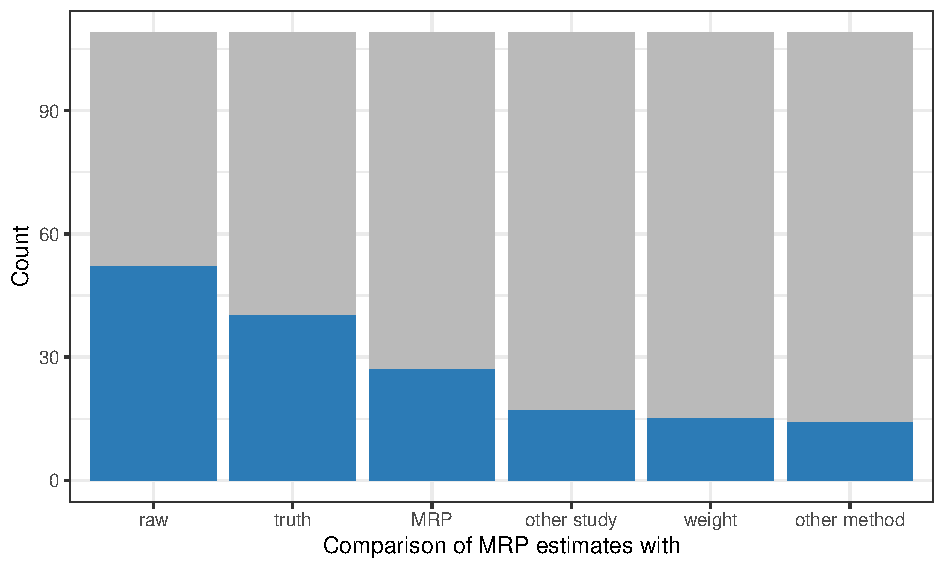
\includegraphics{thesis_files/figure-latex/compare-plot-1.pdf}
\caption{\label{fig:compare-plot}Estimates that are compared with MRP. The blue shade represents the number of articles that compare MRP estimates with the result of other estimation methods, while the grey shade represents the number of articles that also showed comparison of MRP but did not compare to this particular estimate. Note that the blue bars do not sum to the count because some plots compared to multiple alternative estimates.}
\end{figure}

This study finds that from 115 diagnostic plots, 109 (about 95\%) compare MRP estimates with estimates from other methods. Figure \ref{fig:compare-plot} shows the distribution of alternative estimates. MRP estimates are mostly compared to direct estimates and the ground truth. Some studies also compare estimates from several MRP models (usually with different model specifications). There are not many plots showing the comparison between MRP estimates and weighted estimates.

\hypertarget{common-grammar-in-mrp-visualisations}{%
\subsection{Common grammar in MRP visualisations}\label{common-grammar-in-mrp-visualisations}}

\textbf{Plot type}

\begin{figure}
\centering
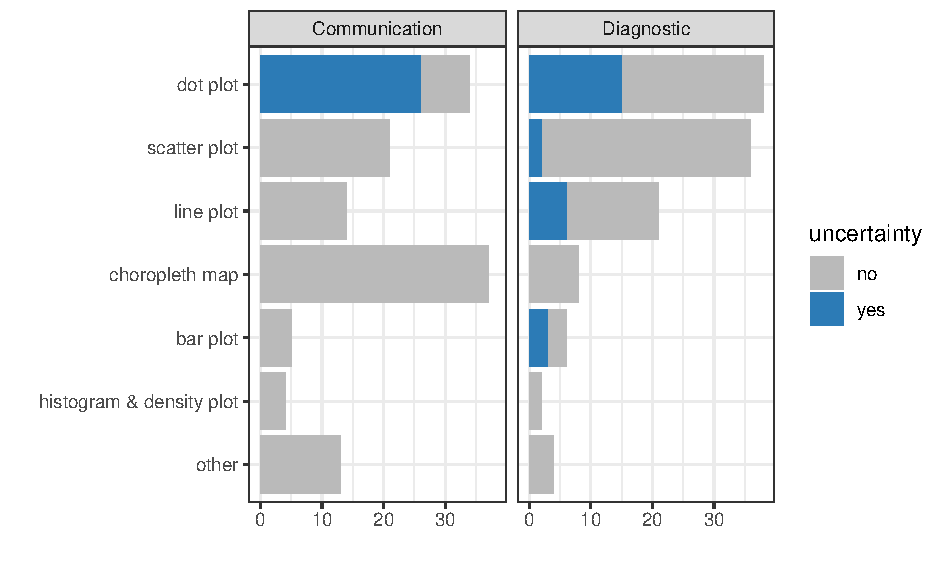
\includegraphics{thesis_files/figure-latex/common-plots-1.pdf}
\caption{\label{fig:common-plots}Common plot types used in MRP visualisations. The blue shade display the number of plots that showed uncertainty, while the grey shade display the number of plots that did not show uncertainty. Both communication and diagnostics plots rarely displayed uncertainty.}
\end{figure}

Plot type, referred to as \texttt{geom} in the grammar of graphics, represents the shape and features displayed in the graph. Figure \ref{fig:common-plots} suggests that communication and diagnostic plots have a different pattern in which plot types are used (See Appendix \ref{terms} for description/definition of each plot type). Communicating MRP estimates are mostly done using a choropleth map as MRP is often used for small area estimation. For diagnostic purposes, dot plots are mostly used to compare more than two estimation methods or to show some performance metrics.

Notice that Figure \ref{fig:common-plots} also displays the use of uncertainty in MRP model visualisations. According to \textcite{MIDWAY2020100141}, displaying uncertainty in the statistical graphs is essential as the absence of this measure would produce a misleading interpretation and hinder some statistical messages. However, he further states that uncertainty is often neglected in data visualisation. This is what we find in this study - uncertainty is not often seen in the plots. This is possibly because many of the application areas are more familiar with official statistics. In official statistics uncertainty is often unreported because results that are not sufficiently precise are not reported.

\textbf{Values put in x and y-axis}

The main component of a data visualisation is the axis. x and y-axis represents what value/data are exactly displayed in the graph. In MRP visualisations (Figure \ref{fig:common-axis}), estimates, small area, actual value (truth), and time are among the values that are displayed in the plot. We can also see that the constructs represented by the x and y-axis are more varied in diagnostic plots. It is worth noting that there are no strict rules on values to put in x and y-axis. However, it is a common that the the fixed value is represented by the x-axis, while the random variable is represented in the y-axis. We do not see this in our results as we find estimates and truth are plotted on the x and y axes interchangeably. Another common rule of thumb is that time is almost always represented on the x-axis, which is supported by the findings of our study.

\begin{figure}
\centering
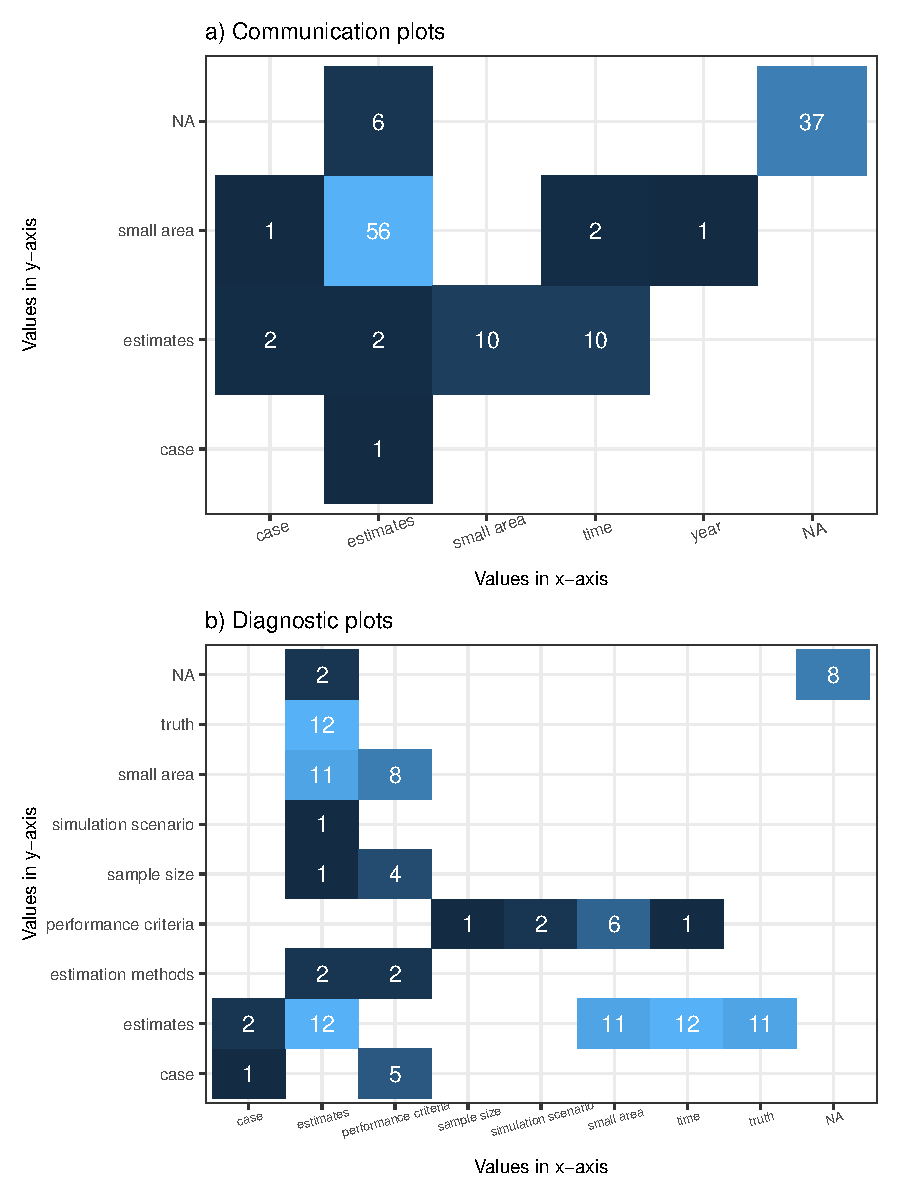
\includegraphics{thesis_files/figure-latex/common-axis-1.pdf}
\caption{\label{fig:common-axis}Common values put in plots' axis. Axis in diagnostic plots more varied compared to communication plot.}
\end{figure}

\textbf{Facet}

Paneling or faceting is considered as to one of the effective visualisation techniques to compare the same variables by its grouping factor \autocite{MIDWAY2020100141}. We find in our results that faceting is a common practice in MRP visualisations. Figure \ref{fig:facet-plots} shows that faceting the plots by small area that is being estimated is the most common, followed by case. Small area refers to the levels of the predictors in the MRP model, for example, state, county, and religion. In several plots, small area could be referred to another variable that is associated with the MRP estimates, but is not included in the model, such as the association between health literacy and the opinion on a health-related bill. Health literacy is a variable that is not included in fitting the MRP model, while the latter is the MRP estimates. Further, case is referred to the outcome predicted with MRP.

\begin{figure}
\centering
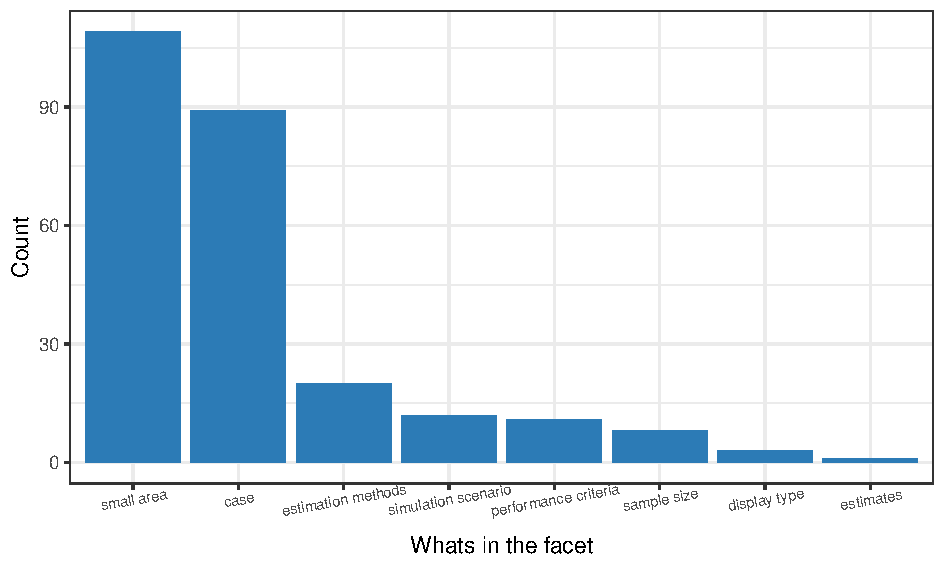
\includegraphics{thesis_files/figure-latex/facet-plots-1.pdf}
\caption{\label{fig:facet-plots}The facetting variable in MRP visualisations}
\end{figure}

\newpage

\textbf{Other features used}

Besides the features explained previously, color and shape are also the components of grammar of graphics. According to a large experimental study on visualisations, color is a memorable feature of a graph \autocite{MIDWAY2020100141}. Further, \textcite{few_2008} states that the aim of color in data visualisations are to highlight particular data, to group items, and to encode quantitative values. In addition, color is sometimes displayed along with shapes to distinguish more features.

We find, as shown in Figure \ref{fig:sankey-feature}, that both communication and diagnostic plots incorporate color only about half the time. Shape is used less often. When there is only one feature to be displayed, for example, estimation methods, people tend to choose to use color first, rather than shape. This is seen in Figure \ref{fig:sankey-feature} as after incorporating color to distinct estimates, small area, estimation methods, and performance criteria, people tend to not use shape anymore.

\begin{figure}
\centering
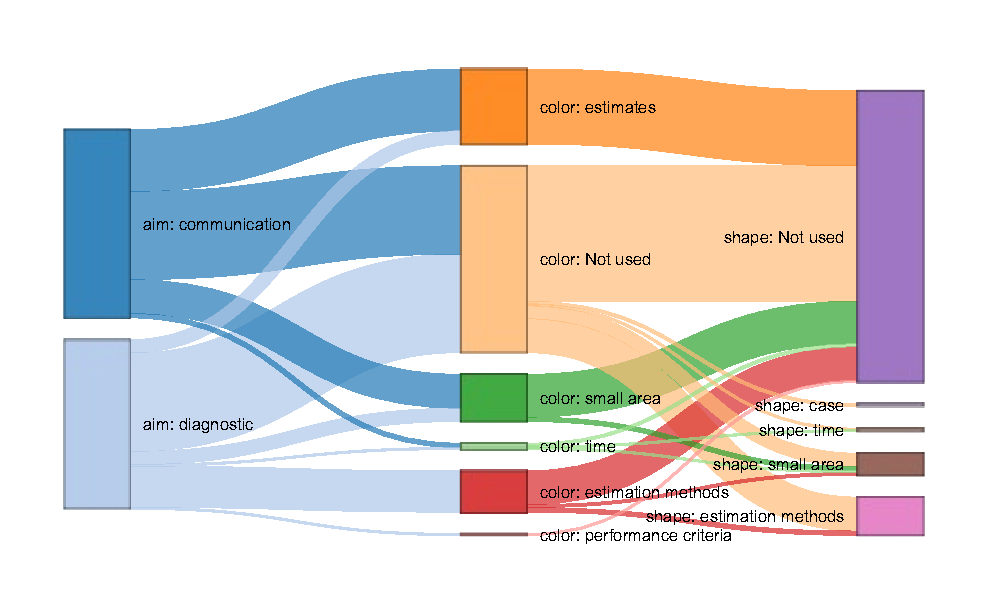
\includegraphics{thesis_files/figure-latex/sankey-feature-1.pdf}
\caption{\label{fig:sankey-feature}Color and shape commonly used in MRP visualisations. Both communication and diagnostic plots rarely use color and shape features.}
\end{figure}

\hypertarget{ch:case-stud}{%
\chapter{Case Study: Application of MRP in Presidential Voting Estimation}\label{ch:case-stud}}

The majority of MRP applications are used in the context of estimating public opinion in the social and political sciences, although, in recent development, MRP is also conducted in various fields, for example, health and environmental studies. When first introduced by \textcite{Gelman97poststratificationinto}, MRP was applied to generate state estimation of the 1988 U.S. presidential election. Additionally, various subsequent studies also made presidential voting the case of interest. We recorded at least seven articles (\textcite{GelmanAndrew2014HBAC}; \textcite{GhitzaYair2013DIwM}; \textcite{KiewietdeJongeChadP2018PSPE}; \textcite{LauderdaleBenjaminE2020Mppf}; \textcite{LeiRayleigh2017T2EA}; \textcite{ParkDavidK2004BMEw}; \textcite{WangWei2015Fewn}) included in the Systematic Literature Review in Chapter 2 have applied MRP in the case of the presidential election. Therefore, in this chapter, we will also apply MRP to estimate the 2016 U.S. presidential voting outcome, especially the probability of voting for Trump. This also allows us to compare MRP estimates with the actual value of the Trump votes that are already available. In this case study, we use the Cooperative Congressional Election Study (CCES) 2016 data \autocite{cces_data} as the survey data and the American Community Survey data 2015-2017 \autocite{acs_data} as the population/ poststratification data.

\hypertarget{data}{%
\section{Data}\label{data}}

\hypertarget{cooperative-congressional-election-study-cces-2016}{%
\subsection{Cooperative Congressional Election Study (CCES) 2016}\label{cooperative-congressional-election-study-cces-2016}}

CCES is an annual survey aims to capture Americans' view on Congress, their voting behavior and experience with regards to political geography, social, and demographic context \autocite{cces_data}. In 2016, CCES covers 64,600 samples spread over 51 states. Accordingly, \textcite{cces_data} mention that the data is precise enough to measure the distribution of voters' preference in most states. In addition, beyond its reliable sample size, CCES is regarded to be desirable dataset as it measures vote preference before and after in two waves so that it is even more reliable compared to generic question \autocite{kuriwaki}.

To fit MRP models, we use several variables from this survey. To obtain the data from the CCES website, we utilize an R package, \texttt{ccesMRPprep} \autocite{ccesmrpprep}. One of the advantages of using this package is that the data has been pre-processed in particular for MRP purposes, in this case, we use the \texttt{ccc\_std\_demographics} function. Also, the variable names are already recoded so it has a more interpretable names. The code to get the data is available in the supplementary materials of this thesis.

The outcome variables, which will be explained in detail in Section \ref{spec}, are the vote preference/intention (\texttt{CC16\_364c}), candidate voted (\texttt{CC16\_410a}), and party identity (\texttt{pid3} including leaners, i.e, coded as Independents in pid3 who expressed leaning towards a party in \texttt{pid7}). Table \ref{tab:outcome-table} shows the distribution of answers in those three variables. In \texttt{ccesMRPprep}, these variables have been renamed so that they are equivalent to \texttt{intent\_pres\_16}, \texttt{voted\_pres\_16}, and \texttt{pid3\_leaner}, respectively. It is worth noting that the MRP models we would like to build use binary responses into yes/no in terms of whether the respondents vote for Trump/Republican or not.

\begin{table}
\caption{\label{tab:outcome-table}Percentage of each answer in CCES 2016. This question will be the MRP models outcome in this case study. Since the model outcome is binary, these answer will be converted to be yes/no in the context of vote for Trump/Republican.}

\centering
\begin{tabular}[t]{lr}
\toprule
Candidate voted & percentage\\
\midrule
Hilary Clinton & 34.27\\
Donald Trump & 29.03\\
Other / Someone Else & 6.26\\
Did Not Vote & 0.13\\
Not Sure / Don't Recall & 0.35\\
\addlinespace
NA & 29.97\\
\bottomrule
\end{tabular}
\centering
\begin{tabular}[t]{lr}
\toprule
Candidate will be voted & percentage\\
\midrule
Donald Trump (Republican) & 29.76\\
Hillary Clinton (Democrat) & 42.57\\
Gary Johnson (Libertarian) & 4.87\\
Jill Stein (Green) & 2.17\\
Other & 2.91\\
\addlinespace
I Won't Vote in this Election & 5.13\\
I'm Not Sure & 10.12\\
NA & 2.47\\
\bottomrule
\end{tabular}
\centering
\begin{tabular}[t]{lr}
\toprule
Party identity including leaners & percentage\\
\midrule
Democrat (Including Leaners) & 48.20\\
Republican (Including Leaners) & 32.27\\
Independent (Excluding Leaners) & 16.24\\
Not Sure & 3.20\\
NA & 0.08\\
\bottomrule
\end{tabular}
\end{table}

Further, the geography and demographic variables used as covariates in the models are \texttt{state}, \texttt{age}, \texttt{gender}, \texttt{education}, and \texttt{race}. Table \ref{tab:covariate-tables} shows the distribution of categories/levels of \texttt{age}, \texttt{gender}, \texttt{education}, and \texttt{race}. Initially, age is a discrete variable but in this case it is categorised. Also, \texttt{education} and \texttt{race} has more levels in the original data but it is collapsed here to obtain fewer levels. The proportion of people answered the survey based on the state is displayed in the appendix of this thesis (\ref{apd-state}).

\begin{table}
\caption{\label{tab:covariate-tables}The response of covariates. Note that this response has been categorised into certain levels that are reflected in these tables.}

\centering
\begin{tabular}[t]{lr}
\toprule
Gender & percentage\\
\midrule
Male & 45.71\\
Female & 54.29\\
\bottomrule
\end{tabular}
\centering
\begin{tabular}[t]{lr}
\toprule
Race & percentage\\
\midrule
White & 69.44\\
Black & 12.00\\
Hispanic & 10.59\\
Asian & 3.53\\
Native American & 0.81\\
\addlinespace
All Other & 3.63\\
\bottomrule
\end{tabular}
\centering
\begin{tabular}[t]{lr}
\toprule
Age & percentage\\
\midrule
18 to 24 years & 8.30\\
25 to 34 years & 19.62\\
35 to 44 years & 15.75\\
45 to 64 years & 38.36\\
65 years and over & 17.98\\
\bottomrule
\end{tabular}
\centering
\begin{tabular}[t]{lr}
\toprule
Education & percentage\\
\midrule
HS or Less & 28.41\\
Some College & 35.38\\
4-Year & 23.04\\
Post-Grad & 13.17\\
\bottomrule
\end{tabular}
\end{table}

\hypertarget{american-community-survey-acs-2015-2017}{%
\subsection{American Community Survey (ACS) 2015-2017}\label{american-community-survey-acs-2015-2017}}

In this study, we use the ACS 2015-2017 data as the poststratification data. The ACS provides annual-basis information about jobs and occupations, demographic and citizenship, educational attainment, homeownership, and other topics \autocite{acs_data_about}. Further, the ACS uses monthly probabilistic samples to produce the annual estimates. It could be understood that the ACS is desirable data to represent the U.S. population since the coverage rate for the 2015-2017 ACS is 92.4\%, 91.9\%, 91.6\%, respectively \autocite{acs_coverage_rate}. It is also implied by \textcite{GaoYuxiang2021IMRa} that the ACS is the most accurate representation of the U.S. population every year. However, it is also worth noting that the ACS coverage do not necessarily match the CCES sample, and therefore, bias might always be presented.

To fit MRP models, we need the individual data of the ACS instead of the aggregated statistics. Hence, we use the 1-year Public Use Microdata Sample (PUMS), which carries the information/records of individual people on a yearly basis. The 1-year PUMS data reflects approximately one percent of the U.S. population \autocite{pums_metadata}. Therefore, in this study, we use three years periods of the ACS 1-Year PUMS from 2015-2017 instead of 2016 only to get a better and more stable representation of the American population. Every individual in the data has a weight (\texttt{PWGTP}). Since we use three years period, this weight is then divided by 3.

The data is publicly available on the \href{https://www.census.gov/programs-surveys/acs/microdata/access.2015.html}{U.S. Census Bureau website}. We downloaded the data in a .csv format (csv\_pus.zip) year by year (2015-2019) through access on \href{https://www2.census.gov/programs-surveys/acs/data/pums/2015/1-Year/}{FTP site}. After that, we did a data pre-processing to bind the three years of the PUMS data. We only use some variables in this data for the MRP-purposes, i.e., unique identifier of the person (\texttt{SERIALNO}), state (\texttt{ST}), weight (\texttt{PWGTP}), education (\texttt{SCHL}), sex (\texttt{SEX}), race (\texttt{RAC1P}), Hispanic origin (\texttt{HISP}), and age (\texttt{AGEP}). We also did a data munging to recode and collapse some categories in these variables. Note that the \texttt{RAC1P} did not record for Hispanic ethnicity. Hence, we introduce a new category here, Hispanic, identified if the person answers other than ``1'' in the \texttt{HISP} variable. Table \ref{tab:acs-response-freq} shows the categorised response of the variables obtained from the ACS, i.e., age, race and ethnicity, and education (see Appendix \ref{apd-state} for state). Also, notice that we get some NA values in education. This is actually the education level of under-school-age respondents. In fact, we will omit the ``Less than 18 years'' age group in the MRP models as it is not included in the survey data (CCES). Hence, the NAs in education response will be eventually omitted as well. The detailed code of the data pre-processing is available in the supplementary materials of this thesis.

\begin{table}
\caption{\label{tab:acs-response-freq}The response categories of post-stratification data.}

\centering
\begin{tabular}[t]{lr}
\toprule
Sex & percentage\\
\midrule
Male & 48.9\\
Female & 51.1\\
\bottomrule
\end{tabular}
\centering
\begin{tabular}[t]{lr}
\toprule
Race and ethnicity & percentage\\
\midrule
White alone & 67.00\\
Black or African American alone & 9.89\\
Hispanic & 14.41\\
Asian alone & 5.16\\
American Indian alone & 0.80\\
\addlinespace
Native Hawaiian and Other Pacific Islander alone & 0.15\\
American Indian and Alaska Native tribes & 0.08\\
Alaska Native alone & 0.07\\
Some Other Race alone & 0.19\\
Two or More Races & 2.24\\
\bottomrule
\end{tabular}
\centering
\begin{tabular}[t]{lr}
\toprule
Age & percentage\\
\midrule
Less than 18 years & 20.73\\
18-24 & 8.73\\
25-34 & 11.92\\
35-44 & 11.62\\
45-54 & 13.45\\
\addlinespace
55-64 & 14.64\\
65-74 & 10.95\\
75-89 & 7.00\\
90 years and over & 0.95\\
\bottomrule
\end{tabular}
\centering
\begin{tabular}[t]{lr}
\toprule
Education & percentage\\
\midrule
No high school & 27.03\\
Regular high school diploma & 18.82\\
Some college & 21.25\\
Associate's degree & 6.39\\
Bachelor's degree & 14.50\\
\addlinespace
Post-graduate & 8.99\\
NA & 3.03\\
\bottomrule
\end{tabular}
\end{table}

\hypertarget{spec}{%
\section{Model Specifications}\label{spec}}

In Chapter 2, we found that the diagnostic plots shown in many articles compare MRP estimates with other estimates, one of which compares several MRP estimates with different specifications. Therefore, in this case study, we build five different MRP models as follows.

\newpage

\textbf{Baseline model}

We begin the model fitting with the baseline model. In this model, we set the binary outcome as whether the respondents vote for Trump or not in the 2016 election. Therefore, we transform the response of \texttt{voted\_pres\_16} into a binary variable called \texttt{vote} ,i.e, if the value of \texttt{voted\_pres\_16} is ``Donald Trump'', then \texttt{vote} variable coded to ``yes'', otherwise ``no''. The NA values in \texttt{voted\_pres\_16} will stay as NA in the new \texttt{vote} variable. Hence, the distribution of the baseline model's outcome variable is displayed in Table \ref{tab:vote-dist}.

\begin{table}

\caption{\label{tab:vote-dist}The distribution of answer in the outcome (vote). It will be the outcome in three models, i.e., baseline model, model with education as additional covariate, and model with more categories in race. We observe a reasonably large percentage of NA.}
\centering
\begin{tabular}[t]{lr}
\toprule
Candidate voted & percentage\\
\midrule
no & 41.00\\
yes & 29.03\\
NA & 29.97\\
\bottomrule
\end{tabular}
\end{table}

The covariates used are \texttt{age}, \texttt{gender}, \texttt{state}, and the re-categorised/collapsed \texttt{race} variable into fewer levels. As seen in Table \ref{tab:covariate-tables}, \texttt{race} has 6 categories, i.e., \texttt{White}, \texttt{Black}, \texttt{Hispanic}, \texttt{Asian}, \texttt{Native\ American}, and \texttt{All\ Other}. In the baseline model, we collapsed the \texttt{Native\ American} and \texttt{All\ Other} into \texttt{Other}. Meanwhile, the levels of \texttt{age}, \texttt{gender}, \texttt{state} stay the same in the levels displayed in Table \ref{tab:covariate-tables}. The baseline model equation is:

\begin{equation} 
\begin{split}
\Pr(vote_{j[i]} = 1) = logit^{-1}\left(\beta_0 + \alpha^{age}_{m[i]} + \alpha^{gender}_{m[i]} + \alpha^{state}_{m[i]} + \alpha^{collapsed\ race}_{m[i]}\right), for\ i = 1, ...., n, 
\end{split}
\label{eq:baseline-model}
\end{equation}

and \(vote_{j[i]}\) is the binary outcome (1 = yes, 0 = no) for individual \(i\) in poststratification cell \(j\). \(\beta_0\) is the intercept. \(\alpha^{age}_{m[i]}\), \(\alpha^{gender}_{m[i]}\), \(\alpha^{state}_{m[i]}\), and \(\alpha^{collapsed\ race}_{m[i]}\) are the random effects for \texttt{age}, \texttt{gender}, \texttt{state}, and \texttt{collapsed\ race}, respectively. The subscript in each coefficient represents the category of the \(i-th\) respondent, such as, \(\alpha^{collapsed\ race}_{m[i]}\) takes value from \{\(\alpha^{collapsed\ race}_{White}\), \(\alpha^{collapsed\ race}_{Black}\), \(\alpha^{collapsed\ race}_{Hispanic}\), \(\alpha^{collapsed\ race}_{Asian}\), and \(\alpha^{collapsed\ race}_{Other}\)\}. Each random effect has an independent prior distribution, such as, \(\alpha^{collapsed\ race}_{m}\) \textasciitilde{} \(N(0, \sigma^2_{collapsed\ race})\) and \(\alpha^{collapsed\ race}_{m}\) \textasciitilde{} \(t(3, 0, 2.5)\). Here, we use the default prior because we only want to compare models for visualisation purpose instead of looking for the best model for estimation.

\vspace{\baselineskip}

\textbf{Model with \texttt{education} as additional covariate}

Next, we create a bigger model by adding \texttt{education} as additional covariate to the baseline model. The levels of \texttt{education} is also displayed in Table \ref{tab:covariate-tables}. Hence, the model specification is:

\begin{equation} 
\begin{split}
\Pr(vote_{j[i]} = 1) &= logit^{-1}\left(\beta_0 + \alpha^{age}_{m[i]} + \alpha^{gender}_{m[i]} + \alpha^{state}_{m[i]} + \alpha^{collapsed\ race}_{m[i]} + \alpha^{education}_{m[i]}\right), \\
for\ i &= 1, ...., n.
\end{split}
\label{eq:model2}
\end{equation}

\vspace{\baselineskip}

\textbf{Model with original race categories}

This model is essentially the same with baseline model, except that there are more race categories, which are \texttt{White}, \texttt{Black}, \texttt{Hispanic}, \texttt{Asian}, \texttt{Native\ American}, and \texttt{All\ Other}. The model equation is:

\begin{equation} 
\begin{split}
\Pr(vote_{j[i]} = 1) = logit^{-1}\left(\beta_0 + \alpha^{age}_{m[i]} + \alpha^{gender}_{m[i]} + \alpha^{state}_{m[i]} + \alpha^{original\ race}_{m[i]}\right), for\ i = 1, ...., n.
\end{split}
\label{eq:model3}
\end{equation}

\textbf{Model with different outcomes}

\textbf{Vote intention/preference}

This model mimicks the model in Equation \eqref{eq:model2}, except that we have different outcome or response variable. The response here is whether the respondent intent to vote for Trump (\texttt{yes}) or not (\texttt{no}). It is transformed from \texttt{intent\_pres\_16} variable in the CCES data to a new variable called \texttt{intent}. If the value of \texttt{intent\_pres\_16} is ``Donald Trump (Republican)'', then \texttt{intent} variable coded to ``yes'', otherwise ``no''. The NA values in \texttt{intent\_pres\_16} will stay as NA in the new \texttt{intent} variable. The distribution of observed ``no'', ``yes'', and NA in this variable is shown in Table \ref{tab:intent-dist}.

\begin{table}

\caption{\label{tab:intent-dist}The distribution of answer in the outcome (intent).}
\centering
\begin{tabular}[t]{lr}
\toprule
Candidate will be voted & percentage\\
\midrule
no & 67.76\\
yes & 29.76\\
NA & 2.47\\
\bottomrule
\end{tabular}
\end{table}

The model is specified as follows:

\begin{equation} 
\begin{split}
\Pr(intent_{j[i]} = 1) &= logit^{-1}\left(\beta_0 + \alpha^{age}_{m[i]} + \alpha^{gender}_{m[i]} + \alpha^{state}_{m[i]} + \alpha^{collapsed\ race}_{m[i]} + \alpha^{education}_{m[i]}\right), \\
for\ i &= 1, ...., n.
\end{split}
\label{eq:model4a}
\end{equation}

\textbf{Party identity}

Beside vote intention, another outcome is the party identity in terms of whether the respondents identify themselves as Republican or not. This variable is derived from \texttt{pid3\_leaner} variable and referred as \texttt{party}. If the value of \texttt{pid3\_leaner} is ``Republican (Including Leaners)'', then \texttt{party} variable coded to ``Republican'', otherwise ``not Republican''. The NA values in \texttt{pid3\_leaner} will stay as NA in the new \texttt{party} variable. The distribution of this outcome variable is displayed in Table \ref{tab:party-dist}.

\begin{table}

\caption{\label{tab:party-dist}The distribution of answer in the outcome (party).}
\centering
\begin{tabular}[t]{lr}
\toprule
Party identity & percentage\\
\midrule
not Republican & 67.65\\
Republican & 32.27\\
NA & 0.08\\
\bottomrule
\end{tabular}
\end{table}

The specification of covariates is also the same with model in Equation \eqref{eq:model2}.

\begin{equation} 
\begin{split}
\Pr(party_{j[i]} = 1) &= logit^{-1}\left(\beta_0 + \alpha^{age}_{m[i]} + \alpha^{gender}_{m[i]} + \alpha^{state}_{m[i]} + \alpha^{collapsed\ race}_{m[i]} + \alpha^{education}_{m[i]}\right), \\
for\ i &= 1, ...., n.
\end{split}
\label{eq:model4b}
\end{equation}

The estimates from the multilevel model is then used for the second stage of MRP, which is poststratification. As the explanation in Section \ref{overview}, poststratification is essentially taking the weight average of the cell-wise posterior estimates with the size of each cell in the population table as the weight \autocite{GaoYuxiang2021IMRa}. For example, the poststratification estimates of Black Men attained High School or less (HS or Less) in Alabama which is categorised in 45 to 64 years old group age who voted for Trump in the 2016 presidential election is:

\begin{equation} 
\begin{split}
\theta_S = \frac{\sum_{j\in S}N_j\theta_j}{\sum_{j\in S}N_j},
\end{split}
\label{eq:poststrat-observed}
\end{equation}

where \(\theta_S\) corresponds to the proportion of 45 to 64 years old of Black Men attained High School or less (HS or Less) in Alabama who respond to ``yes'' in the \texttt{vote} variable and \(N_j\) and \(\theta_j\) are the size of cell corresponds to this sub-population category in the poststratification table and the posterior estimates of this sub-population category, respectively.

\hypertarget{prep}{%
\section{Model Preparation and Fitting}\label{prep}}

The MRP models require a synchronous survey and population data. Hence, to achieve this, we need to map the survey data to the population data. In this study, the model preparation and survey-population data mapping conducted with an R package, \texttt{mrpkit} \autocite{mrpkit}. This package allows the transparent and reproducible workflow to build MRP model, from the data mapping until the prediction stage, including the model specification setting. The detailed code to build the MRP models is available in the supplementary materials of this thesis.

After mapping the survey and population data, we can obtain the poststratification table displayed in Table \ref{tab:post-strat-table}

\begin{table}

\caption{\label{tab:post-strat-table}First five rows of the post-stratification table}
\centering
\begin{tabular}[t]{llllllr}
\toprule
age & state & gender & collapsed\_re & original\_re & education & N\_j\\
\midrule
18 to 24 years & Alabama & Male & White & White & HS or Less & 63982.0000\\
18 to 24 years & Alabama & Male & White & White & Some College & 67957.0000\\
18 to 24 years & Alabama & Male & White & White & 4-Year & 8851.6667\\
18 to 24 years & Alabama & Male & White & White & Post-Grad & 320.3333\\
18 to 24 years & Alabama & Male & Black & Black & HS or Less & 40443.3333\\
\bottomrule
\end{tabular}
\end{table}

Next, we implement Bayesian multilevel model using \texttt{brms} \autocite{brms} to fit the model and obtain the posterior distributions of the parameters. \texttt{brms} itself incorporates cmdstanr \autocite{cmdstanr} as the backend. The samples of posterior distribution are generated in 4 chains with 1000 iterations in each chain. Since this task is computationally heavy and time-consuming, we conduct it using \href{https://docs.monarch.erc.monash.edu/MonARCH/aboutMonArch.html}{Monash's High Performance Cluster (HPC)}.

\hypertarget{results-and-discussion}{%
\section{Results and Discussion}\label{results-and-discussion}}

The MRP estimates from these models will be visualised in this subsection. We will illustrate the implications of current visualisation practices and discuss the possibility for improvement using these estimates. We will divide the discussion with regards to communication and diagnostic plot as we did in in the systematic literature review (Subsection \ref{com-prac}).

\hypertarget{visualisations-for-communication-purposes}{%
\subsection{Visualisations for communication purposes}\label{visualisations-for-communication-purposes}}

One of the most widely used graphs to communicate MRP estimates is a choropleth (see Figure \ref{fig:common-plots}). Choropleth is colored, shaded, or graded to display a spatial pattern of a certain variable. For example, blue and red are used to represent states with more Democrat and Republican voters, respectively, as seen in \textcite{GhitzaYair2013DIwM}. A color gradient is also used to convey a more detailed message, for example, the state-wise MRP estimates of pro-environment opinion as seen in \textcite{EunKimSung2018Epoi}. The greener the shade, the more proportion of people support pro-environmental policy. These two examples also show the use of color with respect to the meaning that people generally perceive, i.e., green is often associated with the environment, and blue is often associated with Democrats.

In this case study, we create a choropleth of MRP estimates of the probability of voting for Trump (\ref{fig:choro}) in the U.S. 2016 election using the baseline model. We create the same choropleth that is commonly shown based on our findings in the literature review.

\begin{figure}
\centering
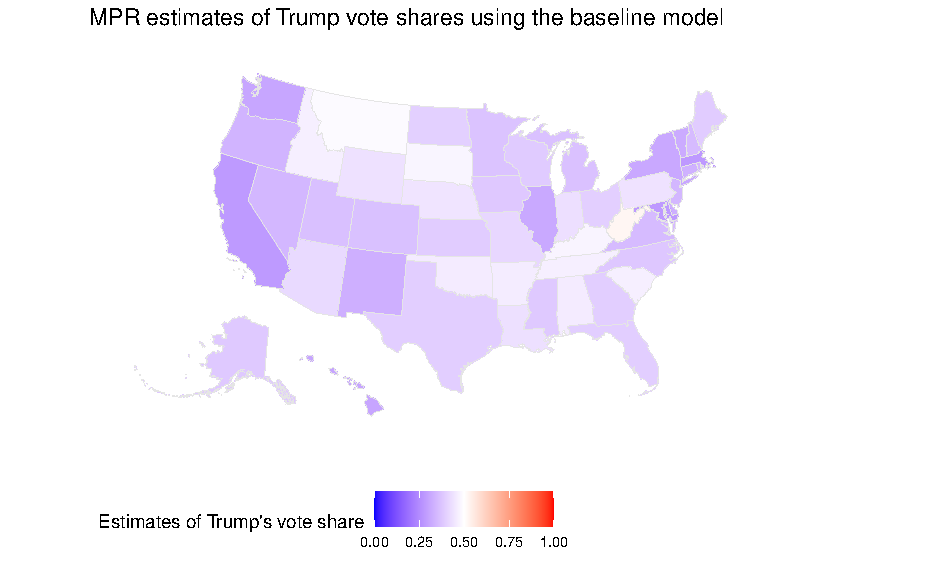
\includegraphics{thesis_files/figure-latex/choro-1.pdf}
\caption{\label{fig:choro}MRP estimates of probability vote for Trump in the U.S. 2016 presidential election by states using the baseline model. The deeper the blue shade the less the Trump's vote share in the corresponding state, while the deeper the red, the more Trump's vote share. It is shown that the baseline model predicts that Trump has less than 50 percent vote share in almost every state in the U.S.}
\end{figure}

The choropleth as seen in Figure \ref{fig:choro} conveys that the baseline model predicts that Trump has less than 50 percent of vote share in almost every state in the U.S. Regardless of whether this model has a good fit or not, the message that this graph tries to convey using a color- code is quite easy to perceive. We can see a blue-shaded U.S. map, meaning that Democrat candidate wins the majority votes in most states. However, such takeaway is general, quite contradictory with the purpose of MRP, which is to give more detailed information about sub-population. From the map, we can see that there is only one state that is nearly red-shaded. However, the readers, especially those unfamiliar with the U.S. map, will probably not know which state it is unless the states are labeled with their name.

Another critic on the choropleth is also stated by \textcite{statgraph}. He argues that choropleth is problematic as polygons with small areas are difficult to observe. In fact, these areas sometimes carry particular information. For example, small geopolitical areas often have a density of population. He then mentions that one alternative to overcome this problem is to replace choropleth with a cartogram in which the area is distorted so that its proportional to the value of the variable it represents. Unfortunately, there is no single visualisation among the articles reviewed that utilize this kind of visualisation.

Choropleth also only displays point estimates, which is not enough. Uncertainty should also be considered when visualising data, particularly estimation results, as there is always variability in there \autocite{tukey,MIDWAY2020100141,HullmanJessica2019IPoE}. In this case, a dot plot with confidence or credible interval could be used to visualise MRP estimates, for example, as seen in \textcite{EnnsPeterK2013POit}. We can see that there is a reasonably high percentage of the usage of dot plot with uncertainty in the articles we reviewed. From 34 dot plots, 26 (about 76\%) of them display uncertainty. However, compared to the overall number of communication plots, the portion of the dot plot with uncertainty is only about 20\%.

\hypertarget{vis-purp}{%
\subsection{Visualisation for diagnostic purposes}\label{vis-purp}}

\textbf{Displaying Comparison}

According to \textcite{tukey}, one of the graphic's purposes is for comparison. In MRP visualisation practice, the estimates from various estimation methods are often compared. Here, we compare state-level MRP estimates with raw and weighted estimates regarding their closeness to the actual Trump's vote shares. The common aesthetic used to display this kind of purpose in the reviewed articles is a scatter plot (around 31\% of the total diagnostic plots).

There is an unwritten ``rule of thumb'' that when displaying two variables in a scatter plot, the horizontal axis displays the predictor, while the outcome is put in the vertical axis \autocite{gelmanunwin}. Regarding MRP visualisation, this ``convention'' could be translated by putting the estimates in the y-axis and the actual value in the x-axis, although the practice is sometimes interchangeable (see Figure \ref{fig:common-axis}). We also observe that some of the reviewed scatter plots show performance metrics, such as RMSE and MAE in \textcite{MengXiao-Li2018Spap}. Hence, in Figure \ref{fig:scatter-est-method}, we also display them. Regarding uncertainty, we find more scatter plots displayed without it (see Figure \ref{fig:common-plots}). Here, we add uncertainty to each point estimates. In addition, we use color-blind-friendly color schemes to distinguish the estimation methods as mentioned by \textcite{vanderplas} and \textcite{statgraph}.

\begin{figure}
\centering
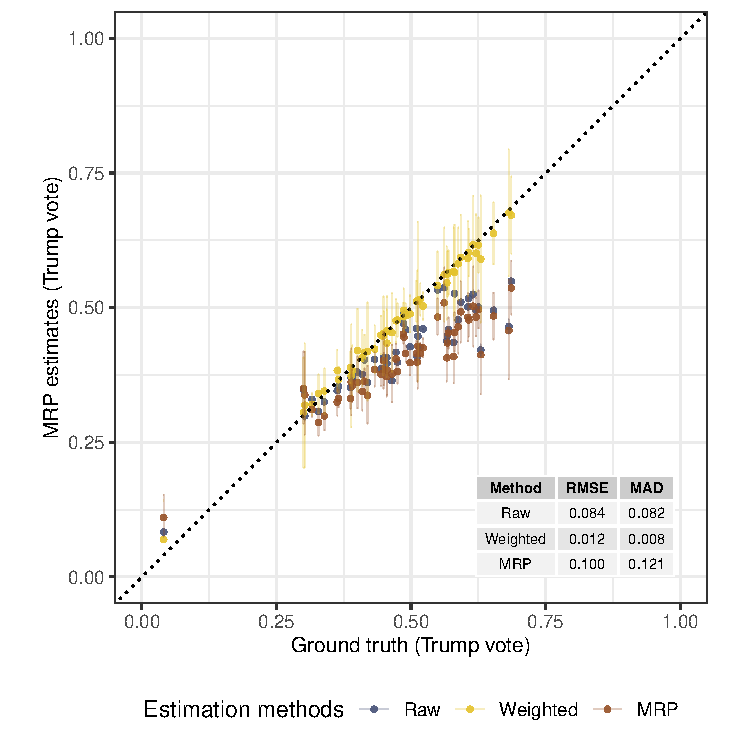
\includegraphics{thesis_files/figure-latex/scatter-est-method-1.pdf}
\caption{\label{fig:scatter-est-method}Comparison between various estimates (raw, weighted, and MRP) with the actual Trump's vote shares. The MRP model used here is the model with education as additional predictor. The points represent states with the 95 percent credible interval, while color represents the estimation method used. Weighted estimates is accurately predict the actual value of Trump's vote shares.}
\end{figure}

Regardless of the visualisation matters, the weighted estimates, as seen in Figure \ref{fig:scatter-est-method}, is observed to be the most accurate estimate. It is actually an expected result, as according to \textcite{cces_data}, the CCES's poststratification weight are weighted to statewide election results. The logic of that one estimate is unbiased, and therefore, some estimates are unbiased also should be kept in mind.

Back to the visualisation matters, a scatter plot is appropriate when the purpose is to allow the readers to discern the general information of the relationship shape between two variables rather than observing individual data points \autocite{saundra}. Hence, if the purpose is to inspect which states are most and least accurately estimated, the scatter plot would not be the graph to use. Giving labels to the points is sometimes observed in practice, but it would be overlapped and hard to read in this case. Again, the dot plot could be used as an alternative to convey state-wise information, as seen in Figure \ref{fig:dot-est-method}. Here, instead of conveying the estimates, we use their deviance from the actual value of Trump's vote share, i.e., the \$Estimates - Actual~value \$. We also display the states in descending order of the actual value of Trump votes, i.e., from the most ``red'' states to the most ``blue'' states.

\begin{figure}
\centering
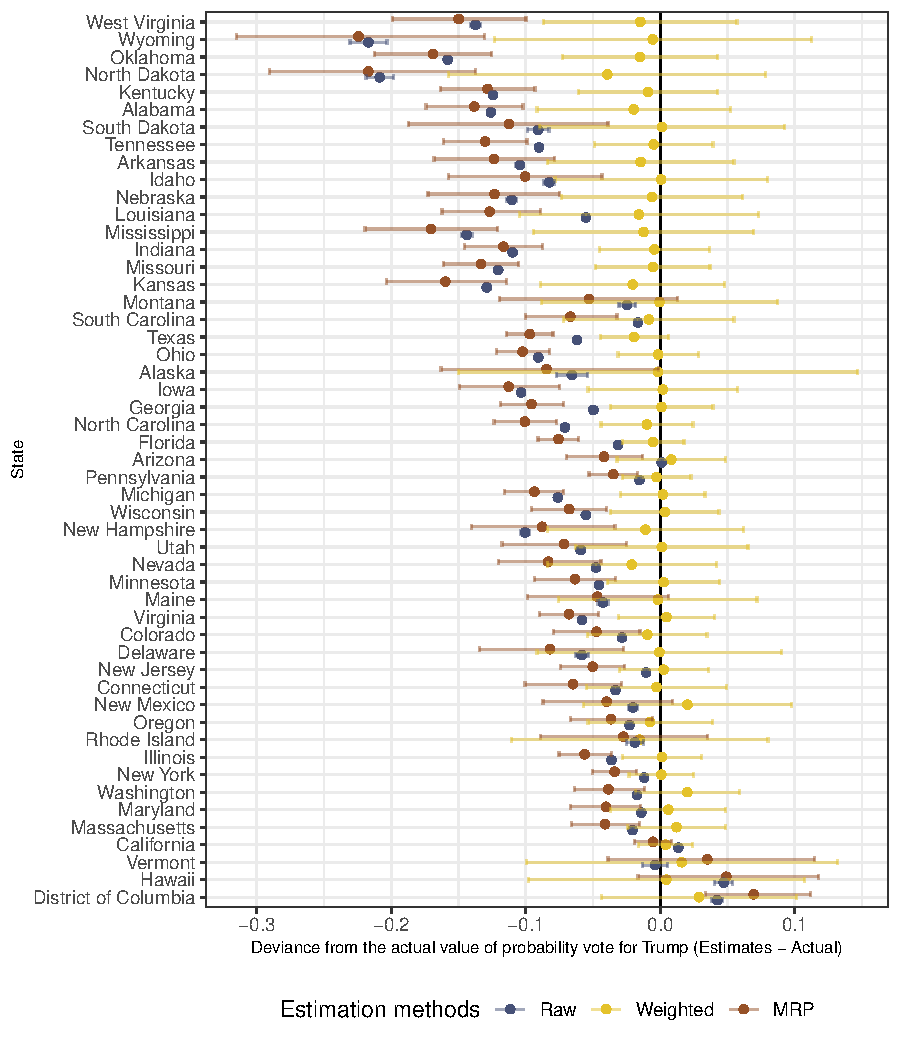
\includegraphics{thesis_files/figure-latex/dot-est-method-1.pdf}
\caption{\label{fig:dot-est-method}The deviance of estimated values from the actual value of Trump's vote shares. The state in the vertical axis are ordered descendingly with regards to the actual Trump vote. The color represents the estimation methods with weighted estimates shows the smallest deviance from the ground truth. This figure shows a pattern in which the more conservative the state, the bigger the deviance.}
\end{figure}

Using this graph, we can get the same information regarding how accurate the estimates are. The advantage of this type of visualization is that it can display other information related to the pattern of estimates, and this pattern is observed in all of the estimation methods. It shows that the more conservative the state, the higher the errors. This pattern can be an indication that the survey data is not enough to capture Trump supporters.

Besides estimation method, comparison could also be made between model specification. Revisiting on what \textcite{WickhamHadley2015VsmR} state, model visualisation could answer how the model fit changes as the data changes. The following graphics will demonstrate this purpose.

As previously, the comparison shown in Figure \ref{fig:state-wise-scatter} is displayed using a scatter plot. The comparison is between the MRP estimates and the actual Trump's vote share. Since there are five model specifications, we use the small-multiple principle \autocite{MIDWAY2020100141}, i.e., displaying the model fits with facets.

\begin{figure}

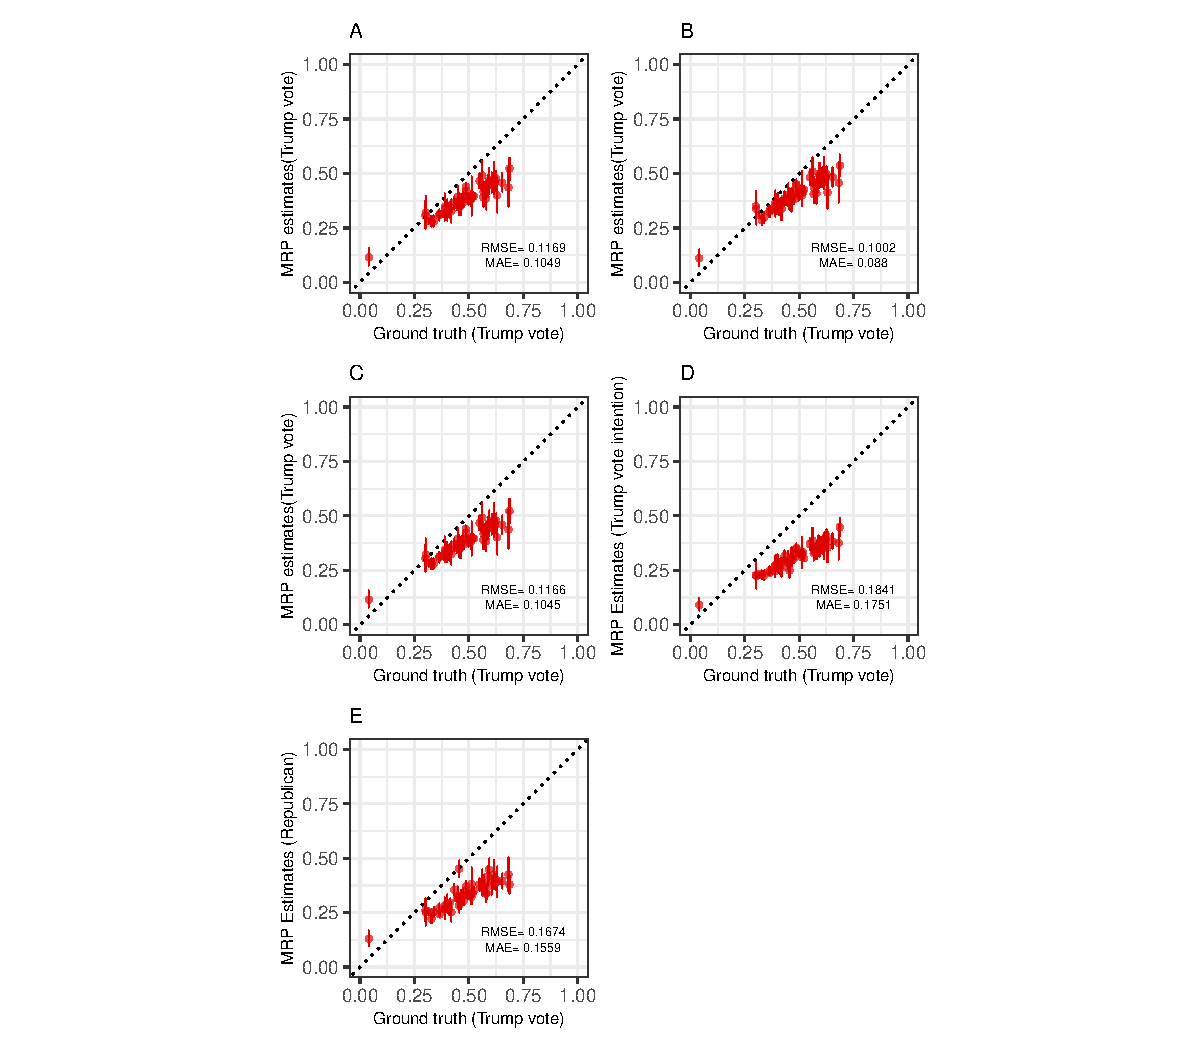
\includegraphics{thesis_files/figure-latex/state-wise-scatter-1} \hfill{}

\caption{Comparison between MRP estimates and the actual Trump's vote share faceted by model specification. The point represents the state. Panel A represents the fit of baseline model; B represents the model with education as additional predictor; C represents the model with more race categories; A, B, and C have the same response variable, vote, while D and E represente the model with different outcome, which are vote intention and party identity, respectively. The covariates used in model D and E are the same with the covariates of model B. We can see that almost all the model fits underestimates the actual Trump's vote share.}\label{fig:state-wise-scatter}
\end{figure}

Using this graph, we can observe that the fit changes as the specification changes. The \(45^{\circ}\) line assists the readers in inspecting whether the fit is underestimated or overestimated. Even though almost all of the fits are underestimated, we can see that the bigger model, i.e., the model with education as an additional covariate, has a better fit than the other models (also shown by its MAE). Model in panels D and E, which are models with different outcomes, are less accurate, which is understandable as the benchmark is the actual Trump vote-share which is more aligned with the other outcome,\texttt{vote}.

In addition to estimation by small geographical area, MRP is also often used to estimate population by demographic subsets. We use violin plots to compare how the subpopulation estimates change as the model specification changes in the following visualisation. We use the violin plot as it can show the distribution of the estimates, although this plot was never observed in the articles we reviewed. It the allows the reader to observe the variability of the estimates, i.e., uncertainty, rather then just the point estimates of summary statistics.

\begin{figure}
\centering
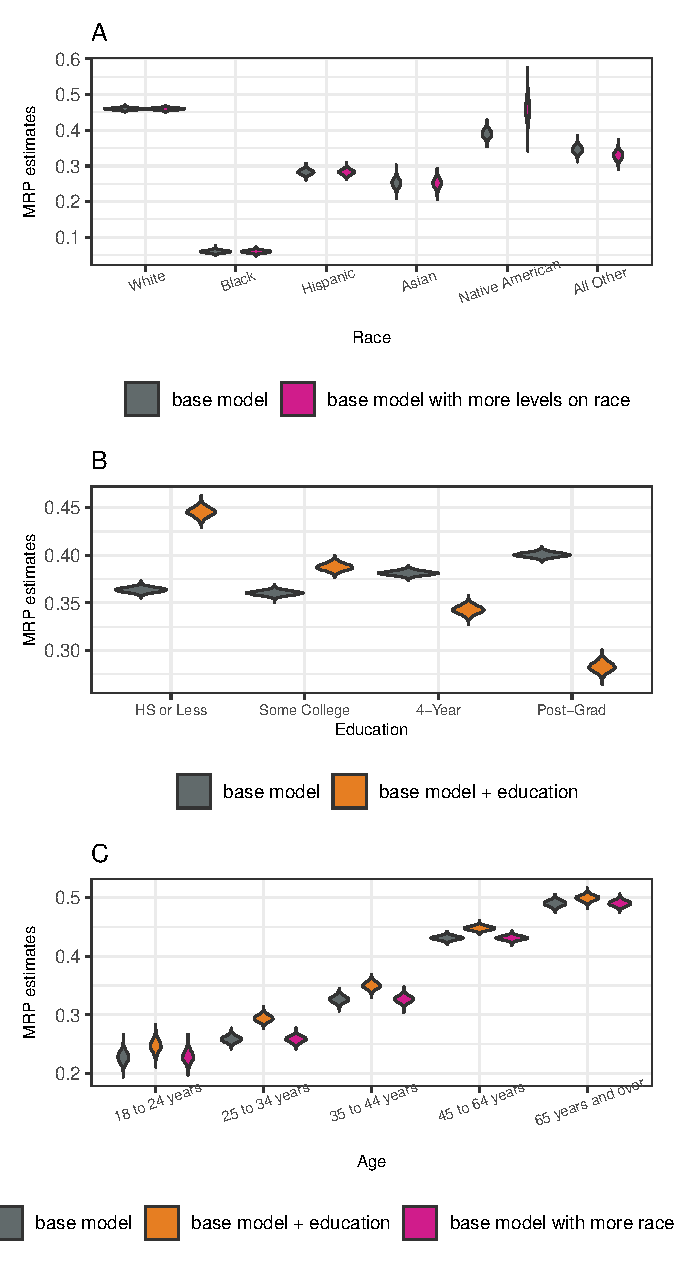
\includegraphics{thesis_files/figure-latex/violin-levels-plot-1.pdf}
\caption{\label{fig:violin-levels-plot}The comparison of MRP estimates by model specification. The panel shows the demographic variables estimated. Panel A, B, and C represents Trump's vote share by race categories, education level, and age group, respectively.}
\end{figure}

Figure \ref{fig:violin-levels-plot} shows the distribution of the response variable, which is probability of vote for Trump for each demographic levels regardless the geographic levels or the states where the voters live. This figure illustrates how the estimates will be different as the result of different covariates used. For example, in Panel A, the range of probability of vote for Trump of Native Americans in the model with more race categories is wider than the model that collapsed Native American and All Other as one race category. We can also see that the median of the outcome in All Other race categories is slightly different in the two models. A more pronounced difference could also be observed in Panel B which compare the baseline model with the model with education level as additional covariate. Incorporating education as covariates results different pattern compared to the baseline model, i.e., the higher the education level, the less probability of voting for Trump. In Panel C, we can see the same trend for the three model fits, i.e., the older age-group tend to vote for Trump. However, the median of model with more covariates is slightly higher in all age group.

\newpage

\textbf{Visualising Metrics}

Metrics are the performance measure of the model in estimating the ground truth. In this case, however, since the benchmark is not the actual value due to the absence of Trump's vote share in demographic levels, the term performance will not be appropriate. We will still display graphs for these metrics, though, as an illustration of performance visualisation.

MAE and bias are predominantly used in most of the articles as the model performance criteria. Essentially, they give the same interpretation, which is how precise the model is in estimating the actual value. We also observe that correlation is frequently used in practice. Some studies also incorporate MSE/RMSE to measure their model performance.

\textcite{WarshawChristopher2012HSWM} display correlation and MAE in a single graph by faceting it. Hence, we make a like-wise plot with a slight modification in the correlation (Figure \ref{fig:cor-race-plot}). The current practices display correlation as it is. When a graph only displays a single metric, there will be no distortion of its interpretation. However, the graph would be quite hard to read if we facet MAE or MSE/RMSE and correlation because of its contradictory interpretation. For MAE and MSE/RMSE, the lower the value, the better the accuracy. In contrast, a higher correlation coefficient is more desirable. Accordingly, in the following graph, we display \(1 - correlation\) instead so that the interpretation is unidirectional. We also set the free ``scale'' so that the consistency of performance of estimates by subpopulation could be examined. Setting the display this way applies the cognitive principle of best graphical practice as stated in \textcite{vanderplas}, in which data is better presented in a way that allows the reader to compare more accurately.

\begin{figure}
\centering
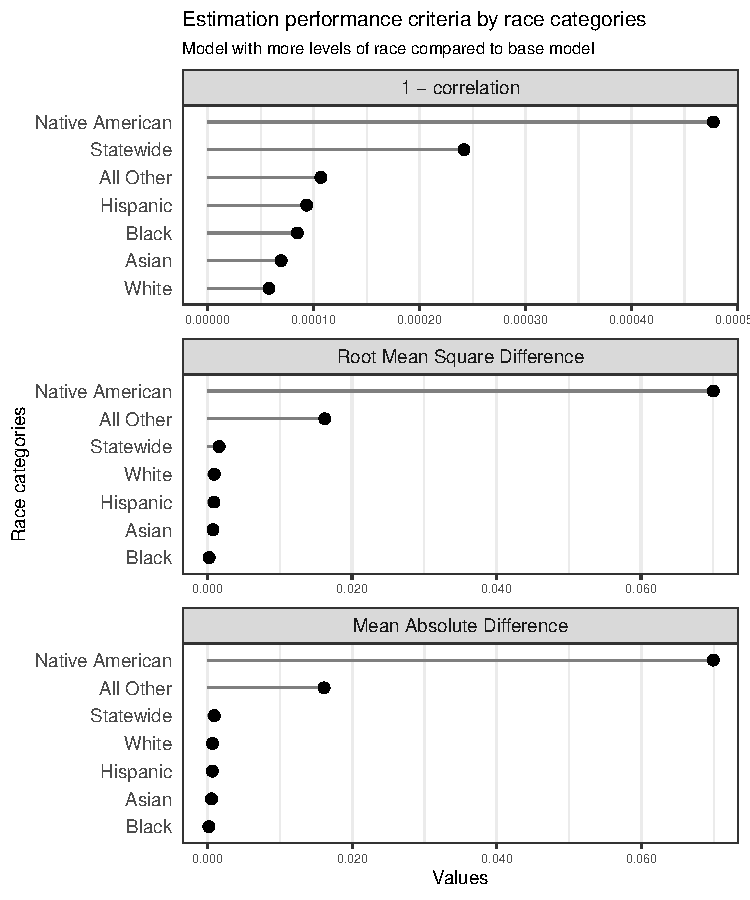
\includegraphics{thesis_files/figure-latex/cor-race-plot-1.pdf}
\caption{\label{fig:cor-race-plot}Metrics of model with more race categories to estimate subpopulation by race categories. This figure in only an illustration as if it used for displaying model performance as the benchmark is the baseline model, not the ground truth. Each panel shows different metrics (Correlation, Root Mean Square Deviance, and Mean Absolute Difference). The statewide categories means the state-wise metrics regardless of the race categories. Native American and All Other are the population subset with the biggest difference to the baseline model.}
\end{figure}

From Figure \ref{fig:cor-race-plot} suggests that Native American and All Other race categories are consistently estimated to have a higher MAD and lower correlation with the baseline model. It is sensible because the baseline model collapses these categories as one covariate. This figure also illustrates how model visualisation answers whether the model is uniformly good or it is only fit for specific regions, in this case, race categories \autocite{WickhamHadley2015VsmR}.

In addition to the metrics displayed in Figure \ref{fig:cor-race-plot}, we also propose alternative metrics that do not exist in the reviewed articles, namely the length of the error bar, in this case, is the 95\% credible interval. It is obtained by subtracting the 2.5\% quantile from the 97.5\% quantile of the estimates. The idea is that there is a bias-variance trade-off in MRP, and metrics, such as MAE, only take bias into account. Therefore, in Figure \ref{fig:race-ci-len}, we display the difference and ratio between the credible interval length of the model with more race categories and the baseline model. This measure will compare the variability of two model fits. If the value of credible interval length difference is near zero, then the variability of two model fits is pretty much the same. The ratio near to 1 could be interpreted in the same way.

\begin{figure}
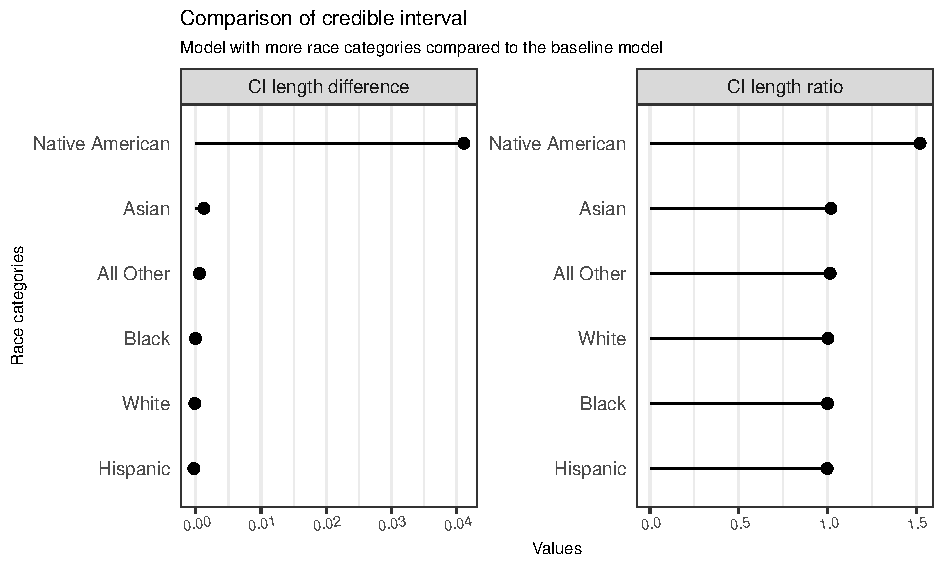
\includegraphics[width=0.9\linewidth]{thesis_files/figure-latex/race-ci-len-1} \caption{Credible interval length comparison between the model with more race categories and the baseline model. The left panel display the mean of length difference, while the right panel display the mean of credible interval ratio. The credible interval length of Native Americans on model with more race categories is 1.5 wider than the baseline model.}\label{fig:race-ci-len}
\end{figure}

Figure \ref{fig:race-ci-len} shows that the estimated interval of Trump's vote share in Native American categories is 1.5 wider compared to the baseline model, while other race categories generally have the same length of the credible interval with the baseline model. Hence, using this type of graph, we can summarise that Native Americans' Trump's vote share more vary than other race categories than the baseline model.

To sum, this demonstration shows that graphical display can help us to understand the model better. For example, the graphs have shown us that the difference in covariates or model specification could result in reasonably different estimates.

\hypertarget{ch:conclusion}{%
\chapter{Conclusion}\label{ch:conclusion}}

Graphics is essential to convey statistical information, and it has been widely used to communicate and diagnose MRP models. However, there have been few studies discussing it. Therefore, in this study, we conduct a systematic literature review to review the current practice in MRP visualisation. In addition, we perform a case study using CCES data to demonstrate the implication of current visualisation practice and explore the alternatives of possible improvement for it.

We find that the choropleth map is the most frequently used visualisation to communicate MRP estimates. However, it is problematic as it often hinders the information in small geographic areas and does not consider the uncertainty of estimates. Hence, we use another option to display state-wise estimates using a dot plot with an error bar. Regarding uncertainty, even though it is important to show estimates variability, it is not much displayed in practice. We offer some alternatives to display it, for example, using a violin plot. This study also demonstrates how graph has aided us in understanding how estimation method and model choices affect the estimates. We also use the credible interval length to illustrate visualisation that takes the bias-variance trade-off into account.

This study, however, only explores the alternative possibility of MRP visualisation improvement. Therefore, using experiment, future study is needed to prove whether these alternatives can communicate the message more effectively and enhance the graphics' interpretability.

\appendix

\hypertarget{appendix}{%
\chapter{Appendix}\label{appendix}}

\hypertarget{supplementary-material}{%
\section{Supplementary Material}\label{supplementary-material}}

All of the codes used to conduct the analysis and produce the report is available in \href{https://github.com/Dewi-Amaliah/MRP_diagnostic_plot}{this Github repository}. Particularly, the code for data wrangling and preparation can be found \href{https://github.com/Dewi-Amaliah/MRP_diagnostic_plot/blob/main/case_study/analysis/cces_acs_wrangling.Rmd}{here}, and the code for MRP preparation and visualisation can be found \href{https://github.com/Dewi-Amaliah/MRP_diagnostic_plot/blob/main/case_study/analysis/mrp_fitting.R}{here} and \href{https://github.com/Dewi-Amaliah/MRP_diagnostic_plot/blob/main/case_study/analysis/mrp_vis.R}{here}, respectively.

\hypertarget{terms}{%
\section{Terms description}\label{terms}}

There are some terms we used in Section \{com-prac\} that the readers might find unfamiliar with, especially in Figure \ref{fig:common-plots}, Figure \ref{fig:common-axis}, and Figure \ref{fig:facet-plots}. Hence Table \ref{tab:terms-desc} displays the description of those terms.

\begin{table}

\caption{\label{tab:terms-desc}Terms description used in Systematic Literature Review result}
\centering
\begin{tabular}[t]{l>{\raggedright\arraybackslash}p{30em}}
\toprule
Term & Description\\
\midrule
dot plot & Data is displayed by point/dot, one of the axis is categorical variable.\\
scatter plot & Data is diplayed by point/dot, both x and y-axis are numeric.\\
choropleth map & Thematic map coloured by the proportion of statistical variable it represents.\\
bar plot & Data is displayed by rectangular bar, one of the axis is categorical variable.\\
histogram & Similar to bar plot but number are grouped into ranges.\\
\addlinespace
density plot & Distribution of numerical variable, the y-axis is the kernel density estimates.\\
other types & Other plot types found in the reviewed articles, but the number is too few to be categorised as one category (boxplot, heatmap, bubble plot, and logit curve)\\
case & The response variable that is estimated. It sometimes displayed as faceted plot, in which each panel represents different outcome/response variable. For example, a graph contains 2 facets, A and B are the MRP estimates for opinion regarding same-sex marriage and abortion, respectively. Hence, A and B are considered as case.\\
small area & Estimates of subpopulation, geographically or demographically, for example estimates by state, county, gender, age group, education level, and religion. In some plots, it could also be another variable associates with the MRP estimates. For example, if MRP estimates used as predictor for another response variable and there is a visualisation display their relationship, then this variable is considered as small area.\\
\bottomrule
\end{tabular}
\end{table}

\hypertarget{apd-state}{%
\section{Proportion of observations by states}\label{apd-state}}

The following plots show the percentage of observations by state in CCES and ACS, respectively.

\begin{figure}
\centering
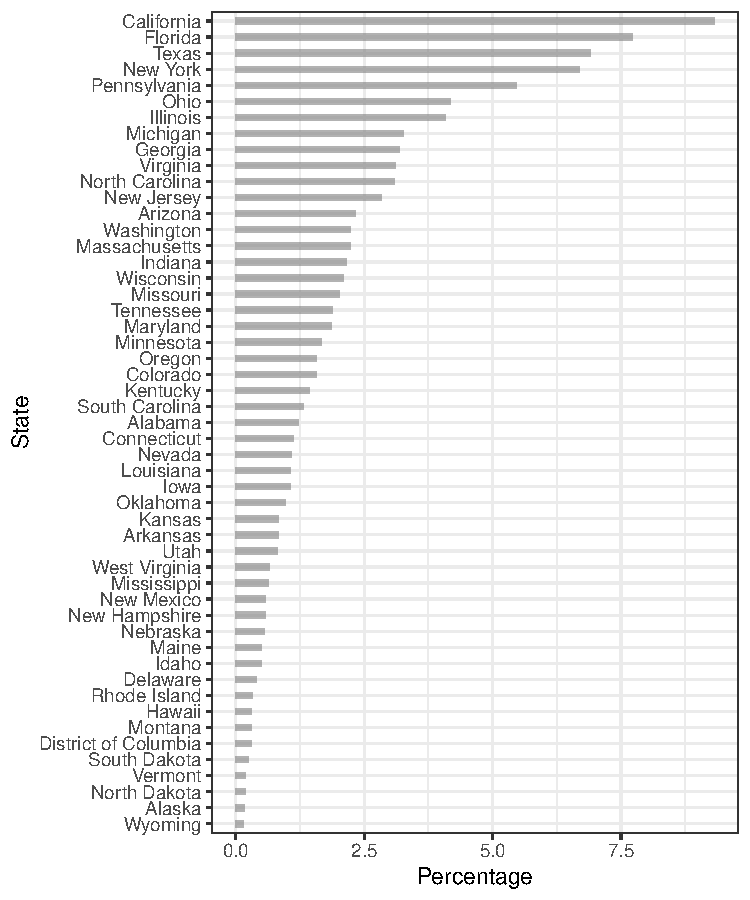
\includegraphics{thesis_files/figure-latex/state-cces-1.pdf}
\caption{\label{fig:state-cces}Distribution of observation in CCES data by state. The horizontal axis represents the percentage of the observations and the vertical axis represents the state ordered from the largest to lowest percentage of observations.}
\end{figure}

\begin{figure}
\centering
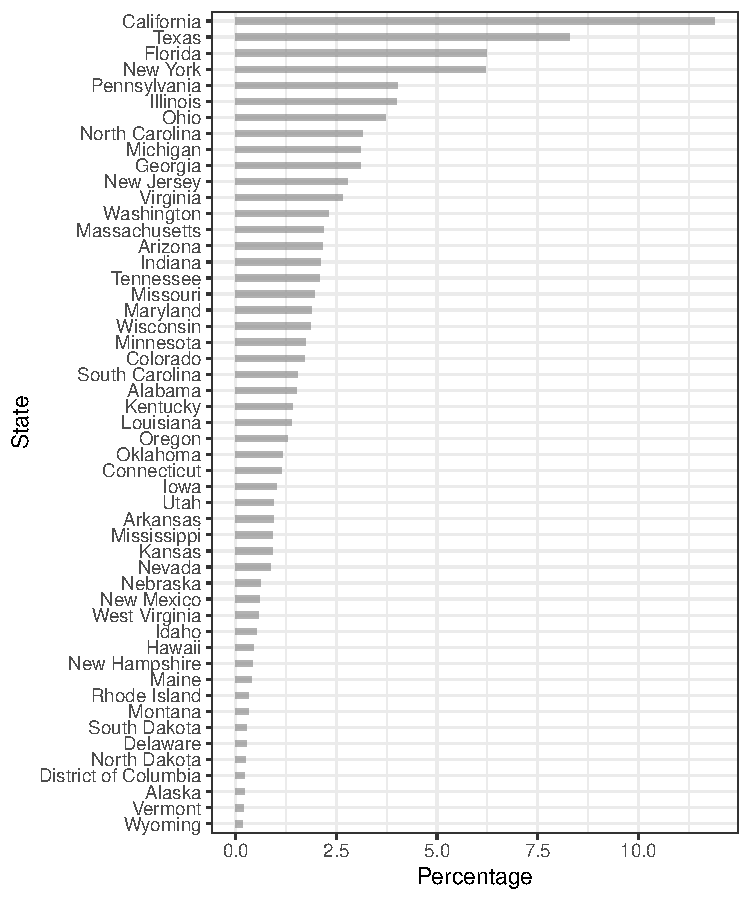
\includegraphics{thesis_files/figure-latex/state-acs-1.pdf}
\caption{\label{fig:state-acs}Distribution of observation in ACS data by state. The horizontal axis represents the percentage of the observations and the vertical axis represents the state ordered from the largest to lowest percentage of observations.}
\end{figure}

\hypertarget{additional-graphs}{%
\section{Additional Graphs}\label{additional-graphs}}

The following plots represent metrics and 95\% credible interval visualisation as done in Section \ref{vis-purp}.

\textbf{Education}

Figure \ref{fig:apd-educ-metrics} shows the metrics and Figure \ref{fig:apd-ci-len-edu} shows the 95\% comparison of credible interval length based on education level.

\begin{figure}
\centering
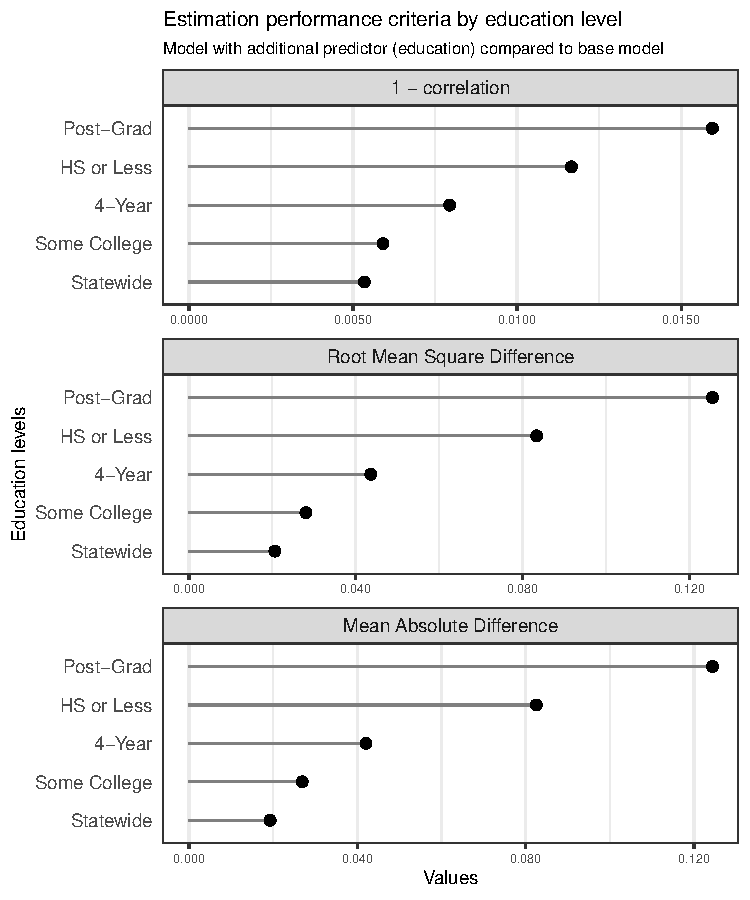
\includegraphics{thesis_files/figure-latex/apd-educ-metrics-1.pdf}
\caption{\label{fig:apd-educ-metrics}Metrics of the model with edication as additional covariate. The benchmark is the baseline model, not the ground truth. Metrics of High school or less and Post-graduate categories are consistently have the higher deviance to the baseline model.}
\end{figure}

\begin{figure}
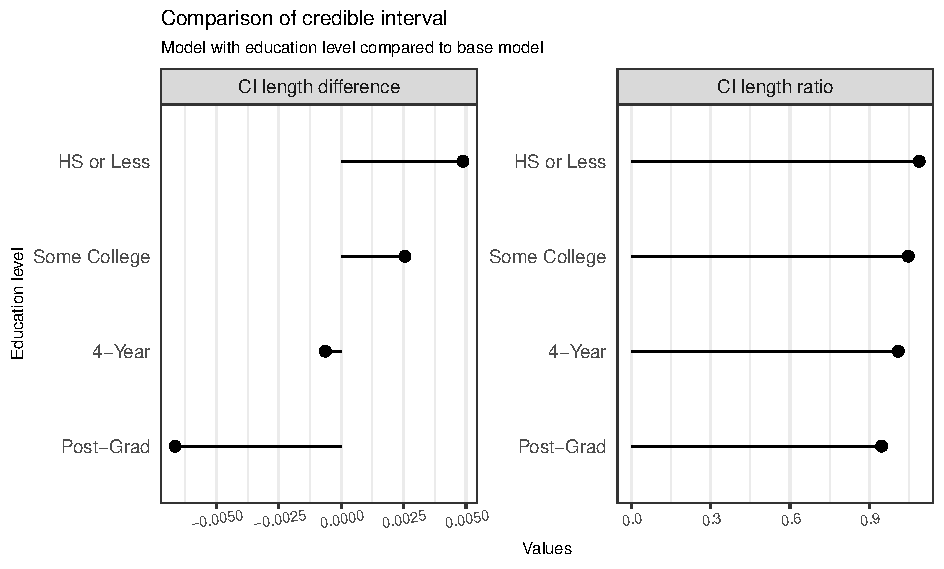
\includegraphics[width=0.9\linewidth]{thesis_files/figure-latex/apd-ci-len-edu-1} \caption{The comparison of the 95 percent credible interval length between model with education as additional covariate and the baseline model by education levels. The credible interval of bigger model for Post-graduate category is slightly narrower compared to the baseline model.}\label{fig:apd-ci-len-edu}
\end{figure}

\newpage

\textbf{Age (The estimation using the model with education as additional covariate)}

Figure \ref{fig:apd-age-fit2} shows the metrics and Figure \ref{fig:apd-age-ci-fit2} shows the 95\% comparison of credible interval length based on age group (the comparison is between the model with education as additonal covariate and the baseline model).

\begin{figure}
\centering
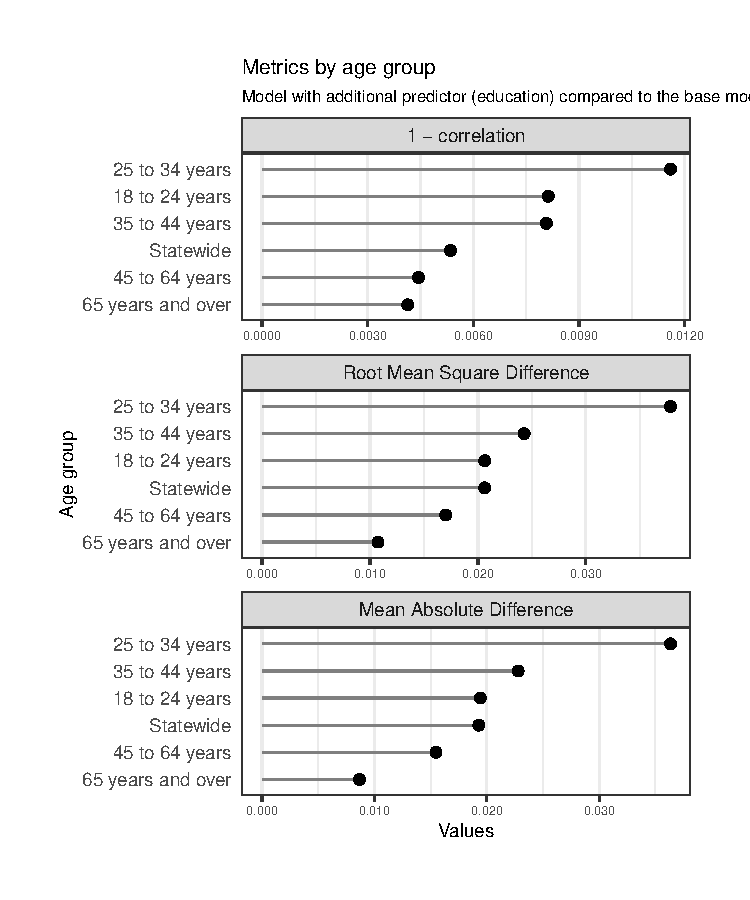
\includegraphics{thesis_files/figure-latex/apd-age-fit2-1.pdf}
\caption{\label{fig:apd-age-fit2}Metrics of the model with education as additional covariate. The benchmark is the baseline model, not the ground truth.}
\end{figure}

\begin{figure}
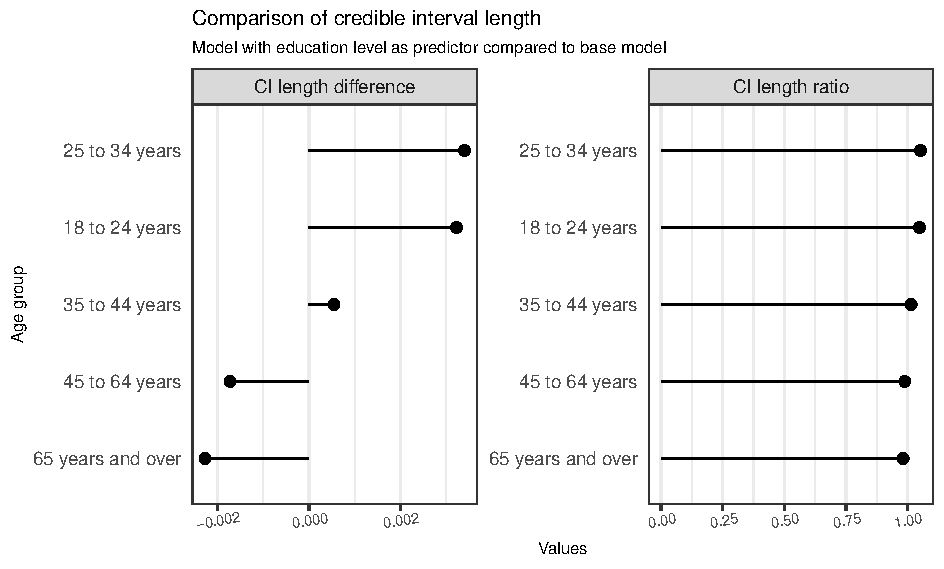
\includegraphics[width=0.9\linewidth]{thesis_files/figure-latex/apd-age-ci-fit2-1} \caption{The comparison of the 95 percent credible interval length between model with education as additional covariate and the baseline model by education levels. The lenght of credible interval between the two model fits is pretty much the same.}\label{fig:apd-age-ci-fit2}
\end{figure}

\newpage

\textbf{Age (The estimation using the model with more race categories)}

Figure \ref{fig:apd-age-fit3} shows the metrics and Figure \ref{fig:apd-age-ci-fit3} shows the 95\% comparison of credible interval length based on age group (the comparison is between the model with more race categories and the baseline model).

\begin{figure}
\centering
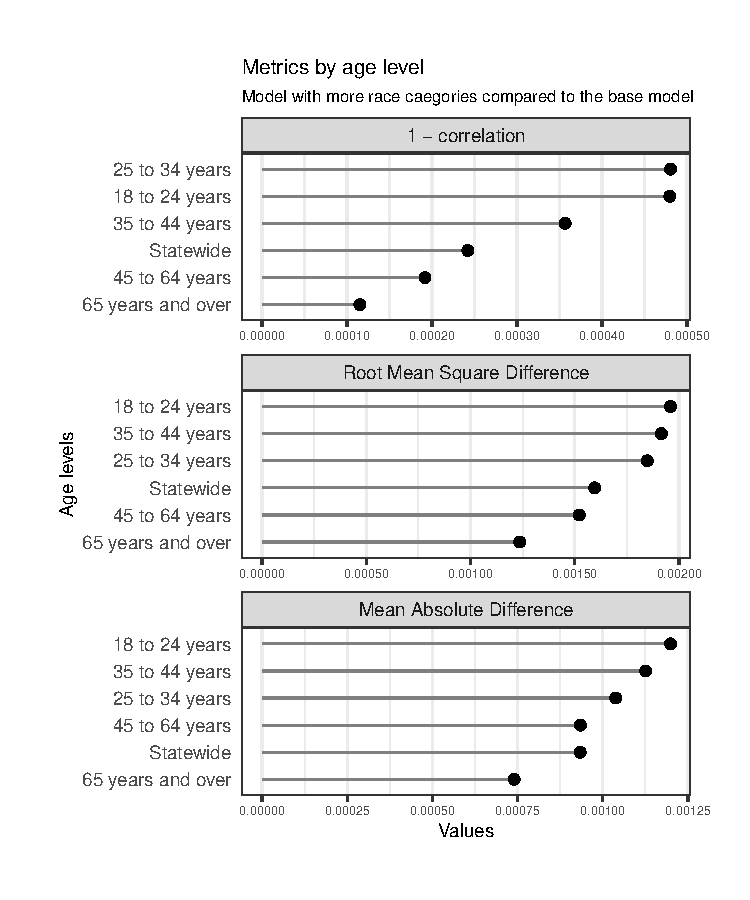
\includegraphics{thesis_files/figure-latex/apd-age-fit3-1.pdf}
\caption{\label{fig:apd-age-fit3}Metrics of the model with more race categories. The benchmark is the baseline model, not the ground truth.}
\end{figure}

\begin{figure}
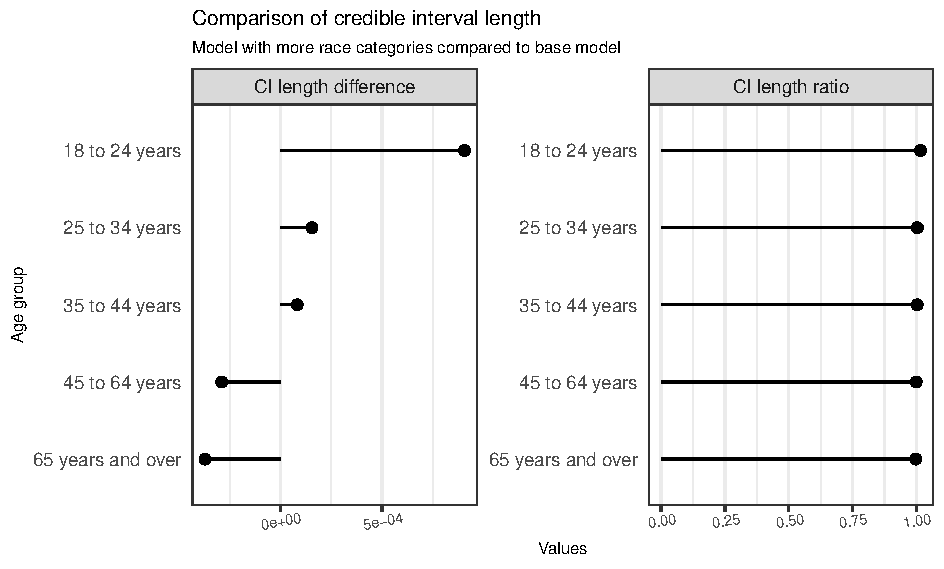
\includegraphics[width=0.9\linewidth]{thesis_files/figure-latex/apd-age-ci-fit3-1} \caption{The comparison of the 95 percent credible interval length between model with more race categories and the baseline model by education levels. The lenght of credible interval between the two model fits is pretty much the same.}\label{fig:apd-age-ci-fit3}
\end{figure}

\printbibliography[heading=bibintoc]



\end{document}
